\documentclass[12pt]{report}
\usepackage{graphicx} % Required for inserting images
\linespread{1.2}

\usepackage[dvipsnames]{xcolor}
\usepackage{tikz}
\usepackage[breakable]{tcolorbox}
\usepackage{colortbl}
\appto{\bibsetup}{\raggedright}

\tikzstyle{mybox} = [draw=RoyalBlue, fill=RoyalBlue!5, ultra thick, rectangle, rounded corners, inner sep=10pt, inner ysep=15pt, text width=0.90\textwidth, align=left] 
\tikzstyle{boxtitle} = [fill=RoyalBlue, text=SkyBlue!30, ultra thick, rectangle, rounded corners, inner sep=10pt, inner ysep=8pt, text width=0.90\textwidth]

\newcommand{\BoxDef}[2]{%
\vspace*{10px}
\noindent

\begin{center}
\begin{tikzpicture}
    \node[mybox](box){\rule{0pt}{30pt}\ignorespaces#2\unskip};
    \node[boxtitle, anchor=north west] at (box.north west) {\textbf{#1}};
\end{tikzpicture}
\end{center}

}

\usepackage[hidelinks]{hyperref}
\usepackage{amssymb}
\usepackage{amsmath}
\usepackage{bm}
\usepackage[top=2.5cm, bottom=2.5cm, left=3cm, right=3cm, centering]{geometry}
\usepackage{algorithm}
\usepackage{algpseudocode}

\begin{document}

\begin{titlepage}
\hrule
\vspace{15pt}
\begin{center}
    \Huge{\textbf{\Huge \textbf{Machine Learning 23-24}} \\ Notes}\\
\end{center}
\vspace{15pt}
\hrule
\vfill
\hrule
\begin{center}
    \Large University of Pisa \\ M.Sc. in Computer Science
\end{center}
\end{titlepage}

\tableofcontents

\chapter{Predictive Models}

The most common framework in ML is to construct \textbf{predictive models} capable of making predictions by looking at a set of data which may be uncertain, noisy, or incomplete. Predictive models are also useful when the theory behind a certain phenomenon is poor or completely absent. ML studies and proposes methods to infer \textbf{functions} from \textbf{examples} of observed data. Such function must:
    \begin{itemize}
        \item \textbf{fit} the example data;
        \item \textbf{generalize} with reasonable accuracy.
    \end{itemize}

A simple example might be recognizing handwritten numbers. The model is presented with some real-life data (pictures of numbers written on paper), and then approximates a function capable of recognizing numbers out of pictures never seen before. 

\section{Components of a Predictive System}

A predictive system can be broken down into the following key components:

\begin{itemize}
    \item Data;
    \item Task;
    \item Model;
    \item Learning algorithm;
    \item Validation;
    \item Prediction.
\end{itemize}

\subsection{Data}

The data represents the available facts. Can be either flat (attribute-value language, fixed-size vector), or structured (more complex data structures).

\textbf{Flat data} can be represented as a table with multiple rows and columns.

\begin{itemize}
    \item Rows: \textbf{examples}, patterns, instances, samples...
    \item Columns: \textbf{features}, attributes, elements, components...
    \item The number of examples is the dimension of the dataset;
    \item The number of features per example is the dimension of the input;
    \item Examples and attributes can be indexed: e.g., $x_i$ is the $i^{th}$ feature of element $x$; \bm$x_i$ is the $i^{th}$ element; $x_{p,i}$ is the $i^{th}$ feature of the $p^{th}$ example.
\end{itemize}

It is often useful to \textbf{encode} the data. Structured data is a complex data structure, such as a list, tree, graph, multi-relational data, etc.

\BoxDef{Noise}{
Noise is the addition of external factors to the stream of information caused by randomness in measurements (which are never always 100\% accurate).
}

\BoxDef{Outliers}{
Outliers are unusual data values, inconsistent with most observations (may be caused by incorrect measurements). They can be removed by appropriate preprocessing (outlier detection).
}

\BoxDef{Feature selection}{
The selection of a subset of features deemed informative. Can provide an optimal input representation for the data.
}

\subsection{Task}

The task defines the purpose of the application: what information do we want to achieve? What can the result be used for? What data is available?

\BoxDef{Supervised Learning}{
\begin{itemize}
    \item \textbf{Given}: a \textbf{training set (TR)} consisting of training examples \bm{$<input,output>$} = \bm{$<x,d>$} (where $d$ is the \textbf{target value}, a categorical or numerical \textbf{label}) for an unknown function \bm{$f$} (called \textbf{target function}).
    
    \item \textbf{Find}: a ``good'' approximation of $f$, called \textbf{hypothesis} \bm{$h$}, that can be used on unseen data to predict its value according to $f$ (= is able to \textbf{generalize}).
\end{itemize}
}
\textbf{Unsupervised learning} is defined the same as the above, but the input data is a TR of unlabeled data.


\BoxDef{Types of tasks}{
\begin{itemize}
    \item \textbf{Classification}: input vectors are seen as members of two or more classes; the goal is to assign a class to any input $x$. The function produces discrete valued outputs (corresponding to the different classes found).

    If the number of classes is 2, the task is binary classification. Otherwise, it's a multi-class problem.

    \item \textbf{Regression}: estimate a real-value function on the basis of a finite set of (noisy) examples.
\end{itemize}
}
These are the two most common supervised tasks. Some other tasks will be seen later.

\subsection{Model}

A model describes the relationships among the data by using a ``language'' (numerical, symbolic,...). The model also defines the set of function the learning machine can implement: the \textbf{hypotheses space H}. 

Many models exist as of today: linear models, symbolic rules, probabilistic models, etc. Why so many? Because \href{https://en.wikipedia.org/wiki/No_free_lunch_theorem}{\textit{there is no free lunch}}: each model is effective and efficient for some problems and not others, has different levels of flexibility, and has different ways to control its complexity.

\subsection{Learning Algorithm}

Given data, task, and model, the learning algorithm executes an \textbf{heuristic search} in the hypotheses space H, in order to find the ``best'' hypothesis that approximates the target function. By ``best'', we mean the function with the \textbf{minimum error}. In order to setup a model, we must make assumptions about the target function, regarding either/both:

\begin{itemize}
    \item Constraints in the model: \textbf{language bias};
    \item Constraints in the learning algorithm: \textbf{search bias}.
\end{itemize}

To explain why such biases are needed, an example is presented.
We want to approximate a boolean function $f$, and we are given a certain number of examples, each of $n$ features, and paired to a label (the output, 0/1). If we want to search for the best approximation of $f$, we would have to search throughout all the boolean functions in the hypotheses space H; the dimension of H is $2^{2^n}$ ($2$ = number of possible outputs, $2^n$ = number of possible inputs). Our function would be essentially \textbf{incapable of generalizing}: if the learner receives an input it already saw, it can classify it, otherwise it can't produce an output (it's a simple lookup table). 

\begin{center}
    \vspace{5mm}
    \boxed{\textbf{NO INDUCTIVE BIAS $\xrightarrow{}$ NO GENERALIZATION}}
    \vspace{5mm}
\end{center}

We can introduce a language bias to limit the number of hypotheses to search through.
For example: let us use conjunctive rules to express the hypotheses (functions can only be propositions connected by the AND operator). The number of total functions that can be expressed in this notation lowers to $3^n + 1$ (total of $n$ possible literals per rule, each literal can be either true, false, or not appear at all; the extra 1 is the hypothesis that always evaluates to false).

\BoxDef{Consistency and version space}{
An hypothesis $h$ is \textbf{consistent} with a training set TR if $h(x)=d$ for each training example $<x,d>$ in TR. The set of all hypotheses in H consistent with a TR is called \textbf{version space (VS)} (can also be referred to as \bm{$VS_{H,TR}$}).
}
Many algorithms exist that can perform a complete search in the hypotheses space H, as in, that are capable of identifying the version space with respect to a TR. However, when using language biases, the restriction of the hypotheses space may be excessive, with the risk of excluding the target function: e.g., referring to the previous example, any rule that uses disjunction (OR operator) would be excluded from the search altogether.

The other approach is to instead use a language capable of expressing all possible hypotheses, and introduce a search bias, using an incomplete search strategy. 

\BoxDef{Loss and error}{
In order to measure the ``goodness'' of an hypothesis $h$, an inner measure is used, called the \textbf{loss function (or loss measure)}: \bm{$L(h(x),d)$}. The expected value of $L$ is called the \text{error} relative to $h$.
}
The loss function and the error can be calculated in any different ways depending on tasks. The following list presents some commonly used loss and error functions (``$w$'' in the error function refers to the vector of parameters that identify that specific $h$).

\begin{itemize}
    \item \textbf{Regression}: predicting a numerical value.
    
    \textbf{H}: set of real-valued funcs.
    
    \textbf{L}: $L(h(x_p),d_p) = (d_p - h(x_p))^2$ (squared error)
    
    \textbf{E}: $E(h_w) = \dfrac{1}{l} \sum_{p=1}^l (d_p - h_w(x_p))^2$ (mean squared error)

    \item \textbf{Classification}: classifying data into two or more classes.

    \textbf{H}: a set of indicator functions (discrete-valued).
    
    \textbf{L}: $L(h(x_p),d_p) = \begin{cases}
                                    0 & \text{if } h(x_p) = d_p \\
                                    1 & \text{otherwise}
                                \end{cases}$
                                    
    \textbf{E}: $E(h_w) = $ mean loss over the data set providing \% of misclassified patterns

    \item \textbf{Clustering}: partitioning data in clusters, each approximated by a centroid/ prototype.

    \textbf{H}: set of vector quantizers.
    
    \textbf{L}: $L(h(x_p), d_p) = (x_p - h(x_p)) * (x_p - h(x_p))$ (squared error distortion)

    \textbf{E}: TBD

    \item \textbf{Density estimation}: estimating density from an assumed class.

    \textbf{H}: set of density functions.

    \textbf{L}: $L(h(x_p), d_p) = -\ln{h(x_p)}$

    \textbf{E}: TBD
\end{itemize}

Error is calculated by measuring loss on new samples of data (a set of labeled examples).

\subsection{Validation}

Validation is the evaluation of performances in ML systems. Any $h$ that approximates the target function $f$ correctly on training examples should also approximate $f$ well on unseen examples.

\BoxDef{Overfitting}{
A learner \textbf{overfits} the data if it outputs an hypothesis $h \in H$ with true/generalization error $R$ and empirical (training) error $E$, but there's a $h' \in H$ with error $R' < R$ and $E' > E$.
}

\begin{center}
    \vspace{5mm}
    \boxed{\textbf{OVERFITTING \underline{DOES NOT} DEPEND ON NOISE}}
    \vspace{5mm}
\end{center}

Overfitting is caused by choosing a model with a complexity such that it adapts too much to the data (noisy data as well), but the presence of noise does not automatically equate to an overfit model.

\BoxDef{Underfitting}{
A learner \textbf{underfits} the data if it outputs an hypothesis with both very high values of generalization error $R$ and empirical error $E$; i.e., the model is too simple to accurately approximate the target function.
}

\section{Statistical Learning Theory}

Statistical Learning Theory (SLT) studies the properties of models to determine their generalization capability, with respect to the training error and underfitting/overfitting zones.

\subsection{VC-bound}

To approximate a target function $f$, the learner must find the hypothesis $h$ with the minimum \textbf{risk function}: \bm{$R = \int L(d, h(x)) dP(x,d)$}, where $P(x,d)$ is a probability distribution. However, when constructing a model, we can only calculate what is the value of the \textbf{empirical risk} \bm{$R_{emp}$} (also called training error E). We can use it to approximate $R$ by indicating an upper bound for it.

Given the \textbf{VC-dim / VC} (Vapnik-Chervonenkis-dim), a measure of the complexity of $H$, then it holds with probability $1-\delta$ the following inequality:

\begin{center}
    \bm{$R \leq R_{emp} + \epsilon(1/l, VC, 1/\delta)$}
\end{center}

Function $\epsilon$ is called \textbf{VC-confidence} and is defined so that it is directly proportional to $VC$, and inversely proportional to $l$ (the dimension of the TR) and $\delta$ (the chosen confidence). With this bound, we can explain undefitting and overfitting in a more formal way:

\begin{itemize}
    \item \textbf{If l is big}: value of $\epsilon$ is low, bound mostly depends of $R_{emp}$ $\xrightarrow{}$ \textbf{enough data to approximate target function};

    \item \textbf{If l is low}: value of $\epsilon$ is high causing the upper bound to increase, regardless of $R_{emp}$ $\xrightarrow{}$ \textbf{too little data to approximate target function};

    \item \textbf{If VC-dim is high}: $R_{emp}$ is low but $\epsilon$ is high, model may be too complex $\xrightarrow{}$ \textbf{overfitting};

    \item \textbf{If VC-dim is low}: $\epsilon$ is low but $R_{emp}$ is high, model may be too simple $\xrightarrow{}$ \textbf{underfitting}.
\end{itemize}
The goal now is to minimize this bound by finding the best trade-off between model complexity and fitting of training data.

\begin{figure}[h]
    \centering
    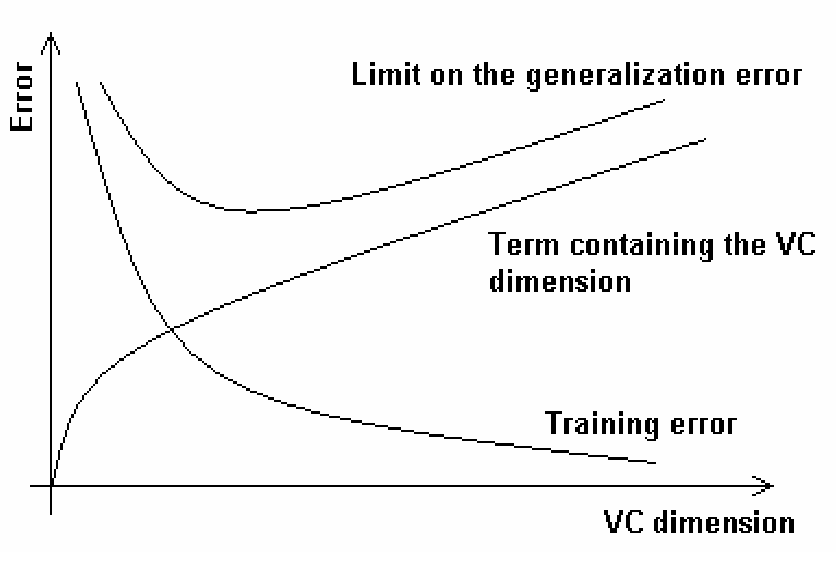
\includegraphics[width=0.5\linewidth]{img/Illustration-of-the-Structural-Risk-Minimization-Principle.png}
    \caption{Graphical visualization of how generalization error and training error vary as the VC-dim of the model changes.}
\end{figure}

\subsection{Validation}

Validation takes place after model training, which determines the weight parameters $w_0, w_1, \dots w_n$ to use for the $h$. The construction of a model can be divided into:

\begin{itemize}
    \item \textbf{Model selection}: estimating the generalization error of different models and choosing the best one (this includes searching for the best hyper-parameters of the model) $\xrightarrow{}$ it returns a model

    \item \textbf{Model assessment}: once a model has been chosen and both parameters and hyper-parameters have been adjusted, evaluating its generalization error on new test data as a way to measure its ``quality'' $\xrightarrow{}$ it returns an estimation
\end{itemize}

Among the different techniques, two simple ones are hold-out cross validation and k-fold cross validation.

With hold-out cross validation, the entire available dataset is divided into three partitions: the training set TR, the validation set VL, and the test set TS. TR is used to run the training algorithm; VL is used to select the best model; TS is used to measure the quality of the final model.

Simple hold-out cross validation can make insufficient use of data. An alternative method is called k-fold cross validation. The dataset $D$ is split into $k$ partitions, $D_1, D_2, ..., D_k$. The training algorithm uses $D/D_i$, and then the validation/test phase is done by using $D_i$. This way all the data is used for both training and validation/testing. The main issues in using this method are choosing the value of $k$, and the fact that's pretty computationally expensive.

\paragraph{Confusion Matrix}
The performance of a classifier can be represented using four counts (True Positives, True Negatives, False Positives, False Negatives), and calculating evaluation measures that summarize the information provided by these counts. The most common measures are:

\begin{itemize}
    \item \textbf{Specificity}: $\dfrac{TN}{FP + TN}$

    \item \textbf{Sensitivity}: $\dfrac{TP}{TP + FN}$

    \item \textbf{Precision}: $\dfrac{TP}{TP + FP}$

    \item \textbf{Accuracy}: $\dfrac{TP + TN}{total}$
\end{itemize}

\begin{figure}[h]
    \centering
    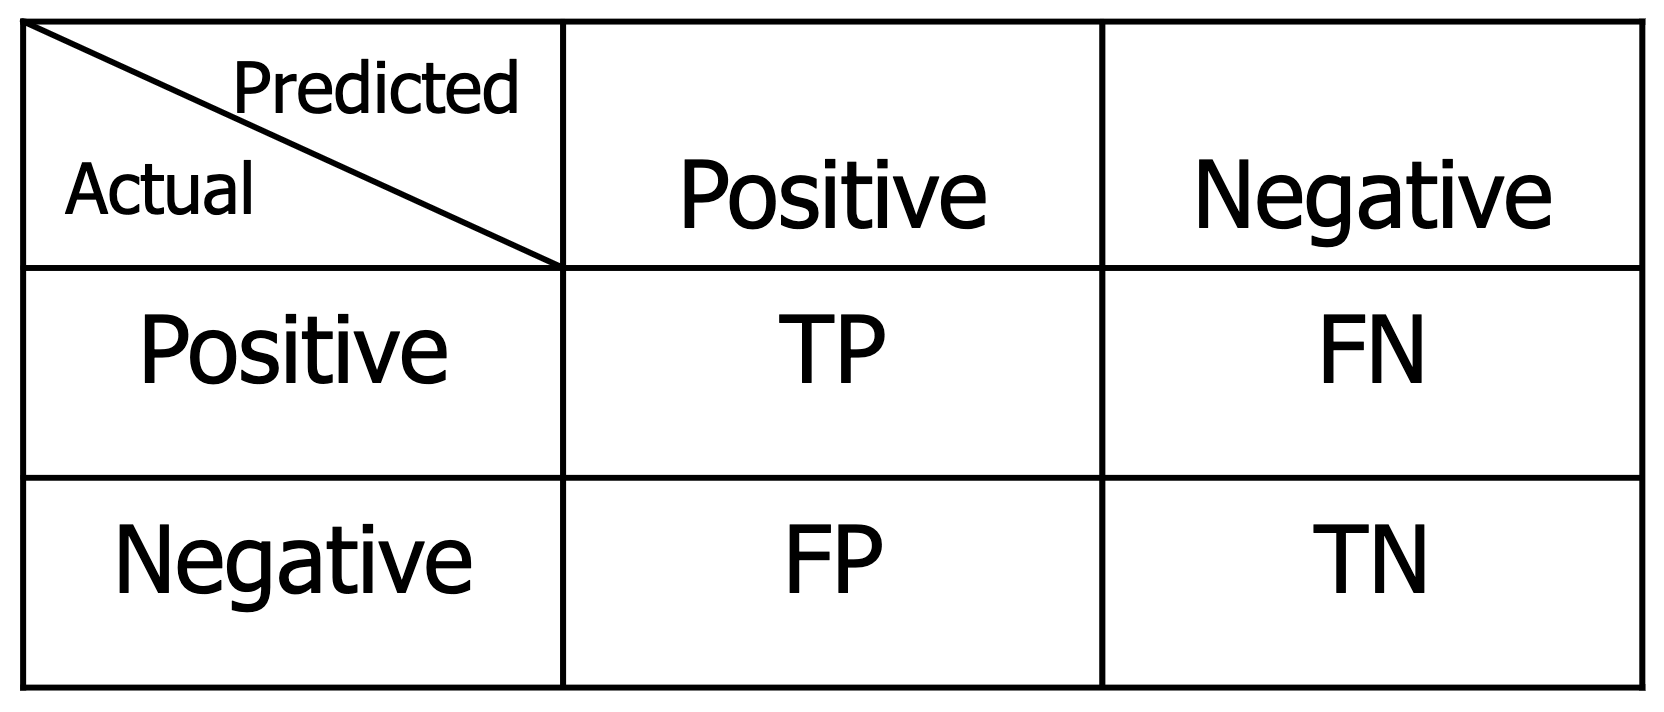
\includegraphics[width=0.5\linewidth]{img/Screenshot 2023-10-04 alle 21.11.26.png}
    \caption{Confusion matrix.}
\end{figure}


\chapter{Linear and K-NN Models}

\section{Linear models}

\subsection{Univariate Linear Regression}

\subsubsection{Unidimensional Input}
The simplest form of regression, with one input variable $x$, and one output variable $y$. We assume a model expressed as:

\begin{equation*}
    h_w(x) = w_1 x + w_0
\end{equation*}

where $w_0$ and $w_1$ are real-valued coefficients (or parameters/weights). This hypothesis corresponds to a simple line. Learning such a function with LMS (least mean squares) means finding the $w$ that minimize the residual sum of squares; i.e., find $argmin_w E(w)$ in $L_2$ (where $E(w) = \frac{1}{l}\sum_{p=1}^l (y_p - h_w(x_p))^2$).

In order to find such value of $w$, we must find the local minimum of the error function, corresponding to the point where the gradient is equal to 0:

\begin{equation*}
    \dfrac{\partial E(w)}{\partial w_i} = 0, i = 1, ..., n+1
\end{equation*}
For the univariate case, $w$ has dimension = 2, so we must search the value of $w$ such that:

\begin{center}
    $\dfrac{\partial E(w)}{\partial w_0} = 0$, $\dfrac{\partial E(w)}{\partial w_1} = 0$.
\end{center}
Below is how the partial derivative of $E(w)$ is calculated for a generic $w_i$:

\begin{equation*}
\dfrac{\partial E(w)}{\partial w_i} = 2 \sum_{p=1}^l (y_p - h_w(x_p)) \cdot \dfrac{\partial (y_p - h_w(x_p)}{\partial w_i} = \boxed{2 \sum_{p=1}^l (y_p - h_w(x_p)) \dfrac{\partial (y_p - w_0 - w_1x)}{\partial w_i}}
\end{equation*}

By calculating for $w_0$ and $w_1$, we get:

\begin{equation*}
\dfrac{\partial E(w)}{\partial w_0} = -2 \sum_{p=1}^l (y_p - h_w(x_p))
\end{equation*}
\begin{equation*}
\dfrac{\partial E(w)}{\partial w_1} = -2 \sum_{p=1}^l (y_p - h_w(x_p)) \cdot x.
\end{equation*}

\subsubsection{Multidimensional Input}
When the input has dimension $n>1$, the function $h_w(x)$ can be expressed as:
\begin{equation*}
    h_w(x) = w_0 + \sum_{i=1}^n w_i x = w_0 + w_1x_1 + w_2x_2 + ... + w_nx_n = \boxed{w^T x + w_0}
\end{equation*}

$w_0$ is often called the \textbf{intercept/threshold/bias/offset...}, since $h_w(x) = 0$ is equivalent to $w^T x = -w_0$.

\subsection{Classification}
The same model(s) used for regression can be used for classification as well. Given a set of $l$ points, equally distributed in two classes, we want to find an \textbf{hyperplane}, represented by $w^Tx + w_0$, that can help decide whether a new point belongs to one class or the other. The function to approximate will be in the form:

\begin{center}
    $h_w(x) = sign(w^Tx + w_0)$\hfill
    \text{or, alternatively,\hfill}
    $h_w(x) = \begin{cases}
                1 & \text{if } w^Tx \geq -w_0 \\
                0& \text{otherwise}
            \end{cases}$
\end{center}
both of whom classify a point depending on where it sits with respect to the defined decision boundary. 

\subsection{Learning Algortihms}

The following section will present two learning algorithms, both using a linear model and based on LMS.
The first algorithm uses a direct approach, based on the normal equation solution. The second algorithm offers an iterative solution based on gradient descent.

The first step is redefining the learning problem and the loss. Assuming a classification problem:

\begin{itemize}
    \item \textbf{Given}: a set of $l$ examples $(x_p, y_p)$, and a loss function $L$

    \item \textbf{Find}: The weight vector $w$ that minimizes the expected loss on the training data $R_{emp} = \dfrac{\sum_{p=1}^l L(h_w(x_p), y_p)}{l}$
\end{itemize}
Let's assume error is being calculated by using least squares (as for the regression), so $E(w) \propto \sum_{p=1}^l (y_p - w^Tx_p)^2$.

The issue with trying to minimize the expected loss is that using a piecewise constant function to calculate it's value can make it a difficult problem, since the function is not differentiable. The solution is to "soften" the loss function by using a smooth, differentiable function instead.

The problem can be reformulated as:

\begin{itemize}
    \item \textbf{Given}: as above

    \item \textbf{Find}: find $w$ to minimize the residual sum of squares:

    $E(w) = \sum_{p=1}^l (y_p - x_p^Tw)^2 = ||y-Xw||^2$,

    where X is a matrix $l \times n$ where each row is an input vector $x_p$.
\end{itemize}

Since this (differentiable) error function is quadratic, the minimum error always exists (but may not be unique). Let's differentiate the function:

\begin{equation*}
\begin{gathered}
    \dfrac{\partial E(w)}{\partial w_j} = \dfrac{\partial \sum_{p=1}^l (y_p - x_p^Tw)^2}{\partial w_j} = 2\sum_{p=1}^l (y_p - x_p^Tw) \cdot \dfrac{\partial (y_p - x_p^Tw)}{w_j} = \\ 2\sum_{p=1}^l (y_p - x_p^Tw) \cdot (\dfrac{\partial y_p}{\partial w_j} - \dfrac{\partial x_{p,1}w_1}{\partial w_j} - \dfrac{\partial x_{p,2}w_2}{\partial w_j} - \dots - \dfrac{\partial x_{p,n}w_n}{\partial w_j}) = \\ \boxed{-2\sum_{p=1}^l (y_p - x_p^Tw)^2 \cdot x_{p,j}}
\end{gathered}
\end{equation*}

The gradient can be also expressed as:
\begin{equation*}
    \dfrac{\partial E(w)}{\partial w_j} = -2\sum_{p=1}^l \delta_p \cdot s_{p,j}
\end{equation*}
This form will be used later.

\subsubsection{Singular Value Decomposition (direct approach)}
We can get the \textbf{normal equation} (the point with gradient of $E$ equal to 0):

\begin{equation*}
(X^TX)w = X^Ty
\end{equation*}
If $X^TX$ is not singular, then the unique solution is given by:

\begin{equation*}
    w = (X^TX)^{-1}X^Ty = X^+y
\end{equation*}
where $X^+$ is the \textbf{Moore-Penrose pseudoinverse} of X.

If $X^TX$ is singular, then the solutions are infinite. The \textbf{singular value decomposition (SVD)} can be used to compute this pseudoinverse:

\begin{equation*}
    X = U\Sigma V^T \implies X^+ = V \Sigma^+U^T
\end{equation*}

where $\Sigma$ is the diagonal, and $\Sigma^+$ is the diagonal where all nonzero entries are replaced by their reciprocal. Moreover, we can apply SVD directly to calculate $w = X^+y$.

\subsubsection{Gradient Descent (iterative approach)}

The \textbf{gradient} is the ascent direction; it expresses in which direction the error function grows. So, by moving with a \textbf{gradient descent}, we can gradually move towards the minimum of the function. The search begins with some initial values given to the weight vector, then the values are modified iteratively to minimize the error function (local search).

\begin{figure}[h]
    \centering
    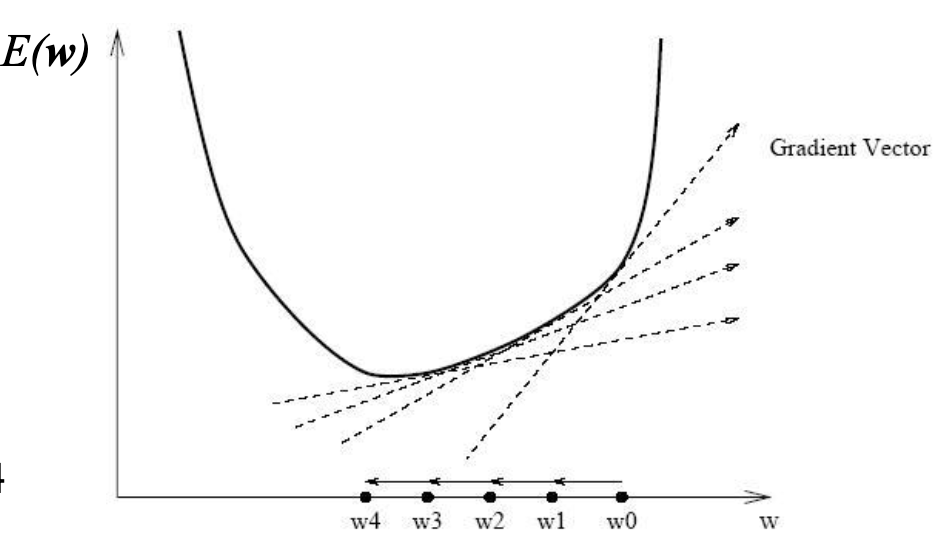
\includegraphics[width=0.5\linewidth]{img/gradient descent.png}
\end{figure}

So, for each iteration, the amount $w$ should be changed with is calculated as:

\begin{equation*}
    \Delta w = - \dfrac{\partial E(w)}{\partial w} =
    \begin{bmatrix}
    - \dfrac{\partial E(w)}{\partial w_1}\\
    - \dfrac{\partial E(w)}{\partial w_2}\\
    \dots\\
    - \dfrac{\partial E(w)}{\partial w_n}
    \end{bmatrix}
    =
    \begin{bmatrix}
    \Delta w_1\\
    \Delta w_2\\
    \dots\\
    \Delta w_n\\
    \end{bmatrix}
\end{equation*}

Each new value of $w$ will be calculated as: $w_{new} = w + \eta*\Delta w$, where $\eta$ is the \textbf{learning rate}: the "step size" that controls the speed of the gradient descent. The algorithm is the following:

\begin{enumerate}
    \item Start with $w_{initial}$ (small), fix value of $\eta \in [0,1]$

    \item Compute $\Delta w = \dfrac{\partial E(w)}{\partial w}$

    \item Compute $w_{new} = w + \eta*\Delta w$

    \item Repeat (2) and (3) until convergence, or $E(w)$ is sufficiently small.
\end{enumerate}
To use least mean squares, divide $\Delta w$ by $l$.

This way of calculating $w$ is called an \textbf{error correction rule} (also called \textbf{delta rule} since it refers to $\delta_p = y_p - x_p^Tw$), since it changes the value of $w$ proportionally to the error to "correct" it:

\begin{itemize}
    \item \bm{$(input_j > 0, error > 0)$} $\rightarrow$ $\Delta w$ is \textbf{+} $\rightarrow$ $w_j$ must be increased $\rightarrow$ increment output $\rightarrow$ \textbf{less error}

    \item \bm{$(input_j > 0, error < 0)$} $\rightarrow$ $\Delta w$ is \textbf{-} $\rightarrow$ $w_j$ must be decreased $\rightarrow$ reduce output $\rightarrow$ \textbf{less error}

    \item \bm{$(input_j < 0, error > 0)$} $\rightarrow$ $\Delta w$ is \textbf{-} $\rightarrow$ $w_j$ must be decreased $\rightarrow$ decrement output $\rightarrow$ \textbf{less error}

    \item \bm{$(input_j < 0, error < 0)$} $\rightarrow$ $\Delta w$ is \textbf{+} $\rightarrow$ $w_j$ must be increased $\rightarrow$ increase output $\rightarrow$ \textbf{less error}
\end{itemize}

This is a simple and effective local search approach to LMS, since it allows us to search through an infinite hypothesis space, and can be applied to models other than linear ones; however, it's not terribly efficient.

\subsubsection{Batch and On-line (stochastic) Gradient Descent}
The \textbf{batch} version of the algorithm, the gradient is calculated as the sum over all $l$ patterns, which provide a more "precise" evaluation off the gradient over the data-set. After the sum, the weights are updated.

The \textbf{on-line} version upgrades the weights with the error computed for each pattern; so, first the weights are updated calculating the error for the $1^{st}$ pattern; those weights are used to calculate the error on the second pattern, updating the weights again; the new weights are then used to calculate the error on the third pattern, and so on. This method can be faster, but needs a smaller $\eta$.

\subsection{Extending the Linear Model}

A problem in $n$ dimensions is \textbf{linearly separable} if it's possible to construct a $n-1$-dimensional hyperplane that separates the points into two groups. The linear decision boundary can provide exact solutions only for these problems.

For example, given 3 points, we can always find a separation plane for every assignment of $f(x)$ (class), save for when all three points are aligned on a straight line and the point in the middle belongs to a different class than the two at the edges:

\begin{figure}[h]
    \centering
    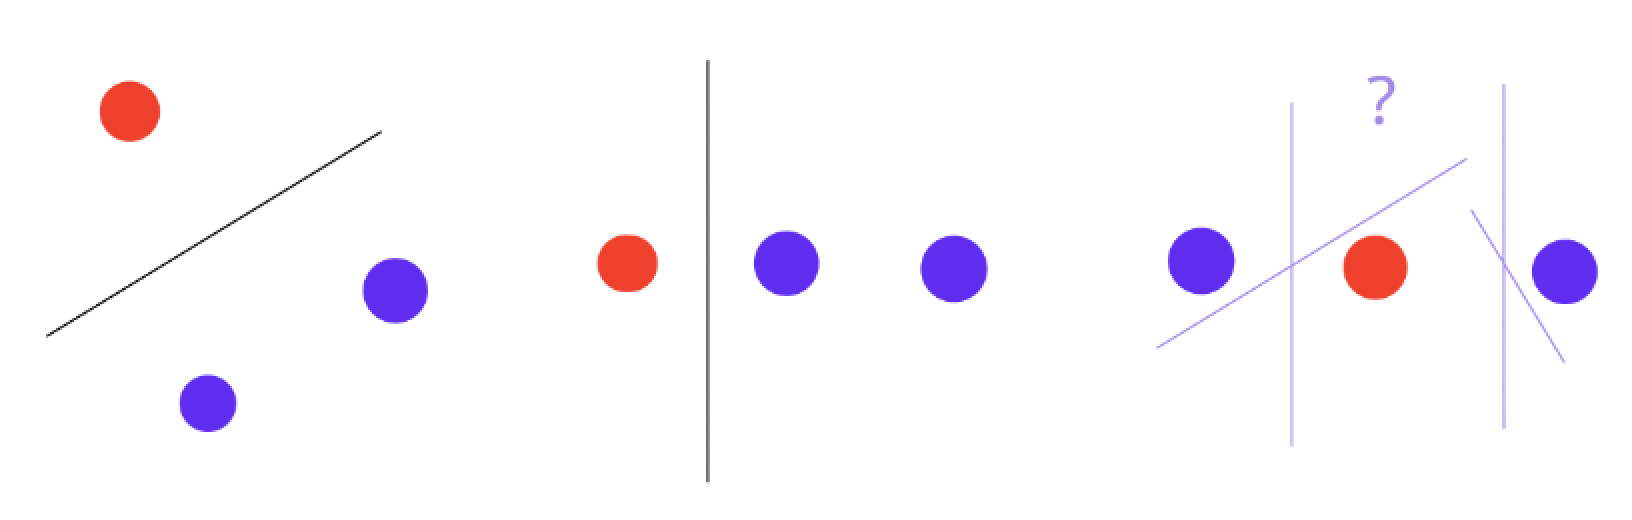
\includegraphics[width=0.6\linewidth]{img/linearly separable.png}
\end{figure}

So, instead of using a linear model, we can use transformed inputs with non-linear relationships with the output, so, for example, we can use a function like the following:

\begin{equation*}
    h_w(x) = w_0 + w_1x + w_2x^2 + \dots + w_mx^m = \sum_{i=0}^m w_ix^i
\end{equation*}

\subsubsection*{Linear Basis Expansion}

This transformation is done by using the \textbf{linear basis expansion (LBE)}:

\begin{equation*}
    h_w(x) = \sum_{k=0}^K w_k\phi_k(x)
\end{equation*}
where each $\phi_k()$ is a function that "transforms" the input; in the previous example, $\phi_0(x)= x^0$, $\phi_1(x)= x^1$, $\phi_2(x)= x^2$, and so on.

Typically, the number of parameters $K$ is greater than $n$.
The model is still linear in the parameters (in $\phi$, not in $x$), so we can still use the same learning algorithm as before, both for regression and classification (by applying the sign function).

\subsubsection{Choosing Phi}
This type of approach is called a "dictionary" approach, since it constructs the linear base expansion out of the function. Using this method can model more complicated relationships (non-linear) since it's more expressive; on the other hand, there's a high risk of overfitting, so we need methods to control the complexity of the model.

\subsubsection{Tikhonov Regularization}
Controlling the complexity can be done in many different ways. One of them is called \textbf{ridge regression (or Tikhonov regularization)}. This method involves adding constraints to the sum of $|w_j|$, penalizing models with high values of $|w|$; i.e., favoring models that use less terms by setting most of the weights to 0 (which results in a simpler model). The loss is calculated as:

\begin{equation*}
    Loss(w) = \sum_{p=1}^l (y_p - x_p^Tw)^2 + \lambda \|w\|^2
\end{equation*}
where $\lambda$ is the regularization hyper-parameter, a small positive value chosen during the model selection phase. Also note that here the name Loss (used for model training) is used to distinguish from Error E (used to evaluate the model error, and corresponding to the data term in this Loss function).

Reformulating the two approaches seen before (direct and iterative), they become as follows:

\begin{itemize}
    \item \textbf{SVD (direct)}: $w = (X^TX + \lambda I)^{-1}X^Ty$

    \item \textbf{Gradient descent (iterative)}: $w_{new} = w + \eta \Delta w - 2\lambda w$ (this is called a weight decay technique; even when the gradient is 0, this addition still reduces the weight by a fraction of it)
\end{itemize}

A balancing can be noted between the value of $\lambda$ and the complexity of the model:

\begin{itemize}
    \item \textbf{Small $\lambda$ value}: the focus is obtaining a small data error term (first term) with a too complex model $\rightarrow $ overfitting;

    \item \textbf{Large $\lambda$ value}: the focus is on the second term, so the data error could grow too much $\rightarrow$ underfitting.
\end{itemize}

The goal is to find the ideal value of $\lambda$ that's neither too small nor too big. We can make a connection between Tikhonov regularization and statistical learning theory; controlling the value of $\lambda$ means controlling the $VC-dim$ of the model, after all: high $\lambda$ means a smaller $VC-dim$ and vice-versa.

\subsubsection{Other Regularization Techniques}

\begin{itemize}
    \item Ridge regression: $\| \|_2$
    \item Lasso: $\| \|_1$
    \item Elastic nets: both $\| \|_1$ and $\| \|_2$
\end{itemize}

The L2 norm penalizes the square value of the weights, and tends to drive all weights to smaller values. L1 norm, on the other hand, penalizes the absolute value of the weights, and tends to drive some weights to exactly 0, but it also introduces a non differentiable loss.

\subsection{Multi-class Task}

\begin{itemize}
    \item \textbf{OVA (one versus all)}: a discriminant function for each class, built on top of real-valued binary classifiers.
    We train $k$ classifiers, each to distinguish the examples in a single class from the examples in any other remaining class; to classify a new example, all $k$ classifiers are run, and the classifier that outputs the largest value is chosen.

    \item \textbf{AVA (all versus all)}: each classifier separates a pair of classes; one classifier for each possible pair. to classify a new example, all the classifiers are run, and the winner is the one with the max sum of outputs or the class with the most votes
\end{itemize}

\section{K-Nearest Neighbor}

The linear model employs an \textbf{eager} learning algorithm: it analyzes the data and constructs an explicit hypothesis capable of generalizing. The final model does not store the training data.

K-Nearest Neighbors instead uses a \textbf{lazy} approach, in which the training data is stored as is; once a new input is presented, it constructs an \textit{ad hoc} hypothesis to classify only that one input.

Its inductive bias is assuming that we can use the distance between points to estimate the output value of a new input.

\subsection{1-Nearest Neighbor}

The simplest possible algorithm. All the training data $TR = <x_p, y_p>$ is stored. Once an input $x$ is received, it finds the nearest neighbor, i.e., the point $x_i$ such that $argmin_i d(x, x_i)$. The distance can be calculated in many different ways (typically euclidean distance). The output for $x$ will be $y_i$, the target value of $x_i$.

This learning algorithm produces a model with no training error, producing decision boundaries that are not linear. Obviously, this leads to overfitting, so the solution is to somewhat increase the training error in order to lessen the generalization error.

\subsection{K-Nearest Neighbors}

Instead of only looking at one neighbor, the output value is calculated by averaging the value of a point's $k$ nearest neighbors. The algorithm first calculates $N_k(x)$, a neighborhood of $x$ that contains $k$ neighbors. Then, the output for regression is calculated as the average target value across that neighborhood:

\begin{equation*}
    h(x) = avg_k(x) = \frac{\sum_{x_i \in N_k(x)} y_i}{k}
\end{equation*}

The output for classification is calculated by majority voting. For a binary classifier it's simply:

\begin{equation*}
    h(x) = \begin{cases}
        1 & avg_k(x) > 0.5 \\
        0 & else
    \end{cases} \, ,
\end{equation*}
or, in the case of multiple classes:
\begin{equation*}
    h(x) = argmax_v \sum_{x_i \in N_k(x)} 1_{v,y_i} \, ,
\end{equation*}
\begin{equation*}
    1_{v,y_i} = \begin{cases}
        1 & v > y_i \\
        0 & else
    \end{cases}
\end{equation*}
The model implicitly uses a \textbf{Voronoi diagram}.

A variant can be used with \textbf{weighted distances}: we may want to add weights to the constribution given by neighbors (i.e. closer neighbors influence the output more than farther ones). So the output for regression is calculated as:

\begin{equation*}
    h(x) = \frac{1}{k}\sum_{x_i \in N_k(x)} \dfrac{y_i}{d(x,x_i)^2} \, ,
\end{equation*}
while the one for classification as:

\begin{equation*}
    h(x) = argmax_v \sum_{x_i \in N_k(x)}  \dfrac{1_{v,y_i}}{d(x,x_i)^2}
\end{equation*}

The main issue in constructing such a model lies in choosing the value of $k$. As seen before, if $k$ is too small, there's overfitting. If $k$ is too big, then both training and generalization errors increase, leading to underfitting.

\subsubsection{Bayes Error Rate}
A Bayes classifier is a learner that uses Bayes' rule to evaluate the most probable output. To find the optimal solution for a classifier, since we know the density $P(x,y)$ (unrealistic situation), we classify to the most probable class: $h(x) = argmax_v P(v|x)$. The error rate of the optimal classifier is called the \textbf{Bayes rate}. It corresponds to the minimum achievable error rate given the distribution of the data.

The K-NN classifier approximates this solution, except that the conditional probability looking at all the data is relaxed to a conditional probability that only refers to a neighborhood of the point, and the actual probability density is unknown.

\subsection{Cons of K-NN}
\begin{enumerate}
    \item \textbf{Scale changes affect the model}: the algorithm does not work as intended is the data is scaled (and thus distances are distorted); the data must be normalized first.

    \item \textbf{High computational cost}: K-NN does not construct a single approximation function; instead, it constructs a new approximation for each input it receives, so the computational cost is completely deferred to the prediction phase. Other than being costly in terms of time (having to calculate distances every time a new input is presented), it's also costly in terms of space, since all the training data must be ready to be used for the prediction.

    \item \textbf{Little space for interpretation}: it's heavily dependent on the metric used.

    \item \textbf{Curse of dimensionality}: as the dimensionality of the data increases, the sparser it becomes, and in turn, the harder it becomes to find the neighbors of a point; and even if found, they would be so far away that the resulting estimate would be no longer local. This would push towards lowering the value of $k$ (so that the estimate depends on closer points), but at the risk of running into overfitting.

    Another relevant issue is that the sampling density ($\frac{l}{volume}$) is proportional to $l^{\frac{1}{n}}$; so, as the dimension grows, the number of points needed to estimate the same function exponentially increases as well.

    Finally, if the target depends only on few of the many features, the output could be influenced by the irrelevant features. This can be solved by either weighting features depending on their relevance, or do feature selection.
\end{enumerate}

\section{Linear Model vs. K-NN Model}

The two models can be considered two extremes:

\begin{table}[h]
    \centering
    \begin{tabular}{c|c}
         Linear & K-NN \\
         \hline
         Rigid & Flexible \\
         Eager & Lazy \\
         Parametric & Instance-based \\
    \end{tabular}
\end{table}

In conclusion, we can say that low variance/ rigidity is poor, but too high variance/ flexibility is dangerous.
\chapter{Neural Networks}

(Artificial) neural networks are a flexible machine learning tool capable of approximating functions with special properties. They can learn from examples, are universal approximators (\href{https://en.wikipedia.org/wiki/Universal_approximation_theorem}{Cybenko's/Universal approximation Theorem}), can deal with noisy and/or incomplete data, and can handle both continuous real and discrete data. Neural networks encompass a wide set of models.

\section{Artificial Neurons}

Artificial neural networks are made up of several \textbf{nodes} (also called artificial neurons or units) connected in a net capable of solving artificial intelligence problems. They are heavily inspired by biological neural networks, down to how the single units work and communicate with each other to learn a certain function.

The main ideas that these models are based on are:

\begin{itemize}
    \item \textbf{Strength reinforcement}: stimuli ``reinforce'' the weights;

    \item \textbf{Plasticity}: the nervous system is highly capable of adapting.
\end{itemize}

Each neuron $i$ has a number of \textbf{inputs} coming from external sources or other units, and corresponding \textbf{weights}, the free parameters that can be modified during the learning phase. Each neuron calculates its \textbf{net input} (weighted sum of inputs) and its output as follows:

\begin{equation*}
    \begin{cases}
        net_i(x) = \sum_j w_{ij} x_j \\
        o_i(x) = f(net_i(x)),
    \end{cases}
\end{equation*}
where $f$ is the unit's \textbf{activator function}.

Note that $w_{ij}$ is the weight of the input coming from the node $j$ and going into the node $i$; some books/libraries/simulators, etc. may use the opposite notation.

\begin{figure}[h]
    \centering
    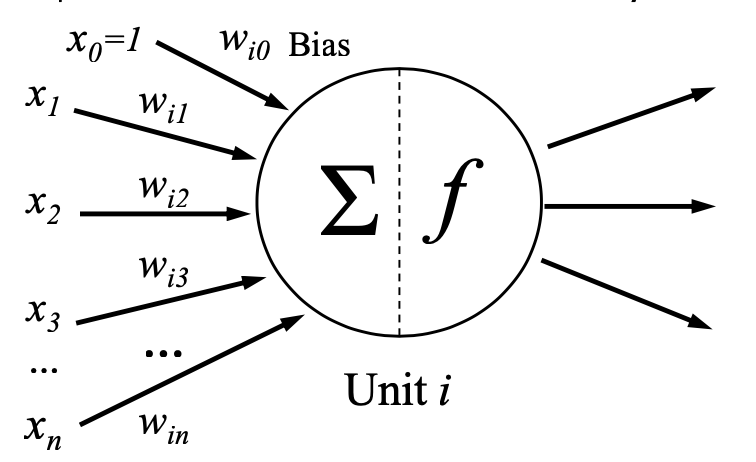
\includegraphics[width=0.5\linewidth]{img/Neuron.png}
\end{figure}

Some examples of activator functions include:

\begin{itemize}
    \item the \textbf{linear activation function};
    \item the \textbf{perceptron/threshold activation function};
    \item the \textbf{sigmoid/logistic function}.
\end{itemize}

\subsection{Perceptrons}

The perceptron was proposed and implemented in 1958 by Frank Rosenblatt. The first perceptron was an actual physical machine designed for image recognition, and not a program. It had a few hundreds of photocells, randomly connected to a layer of neurons.

Multiple perceptrons can be composed and connected to build a network. This is called a \textbf{multi-layer perceptron neural network (MLP NN)}. 

McCulloch and Pitts proposed a neural network model in 1943. In this model, each neuron is in one of two possible states: firing (1), or not firing (0). All synapses (connections) are equivalent and characterized by a weight $w_i$ which is positive for ``excitatory'' connections, and negative for ``inhibitory'' connections. A neuron $i$ becomes active when the sum of the connections coming from other active neurons and the bias is larger than 0. Both inputs and outputs are binary, so it can implement binary classification tasks.

This model essentially describes neurons as perceptrons. The following pictures illustrate how this model can be used to represent boolean functions AND and OR by using a single neuron. Each neuron has two inputs, plus a bias ($w_0$). Both problems are linearly separable, so if the inputs are represented graphically on a plane, we can draw a single line (described by the net function) that separates all inputs that produce a 0 from all the ones that produce a 1.

\begin{figure}[h]
    \centering
    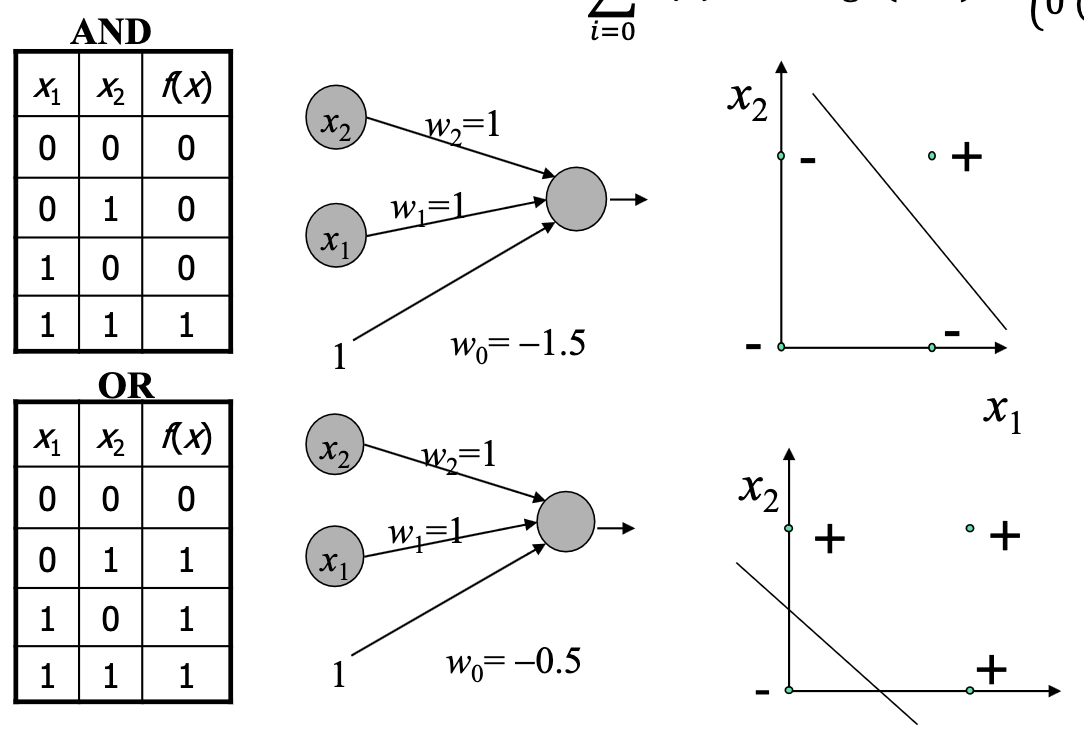
\includegraphics[width=0.5\linewidth]{img/boolean perceptron.png}
\end{figure}

If we instead consider the XOR operator, it corresponds to a non-linearly separable problem, so we can't use a single neuron. The solution is to use a two layer network. The operation can be rewritten as follows:

\begin{equation*}
    x_1 \oplus x_2 = x_1 \cdot \Bar{x_2} + \Bar{x_1} \cdot x_2
\end{equation*}
then we have:
\begin{equation*}
    x_1 \oplus x_2 = \Bar{h_1} \cdot h_2
\end{equation*}
So the XOR operation is moved to a new space that represents the problem as linearly separable:

\begin{figure}[h]
    \centering
    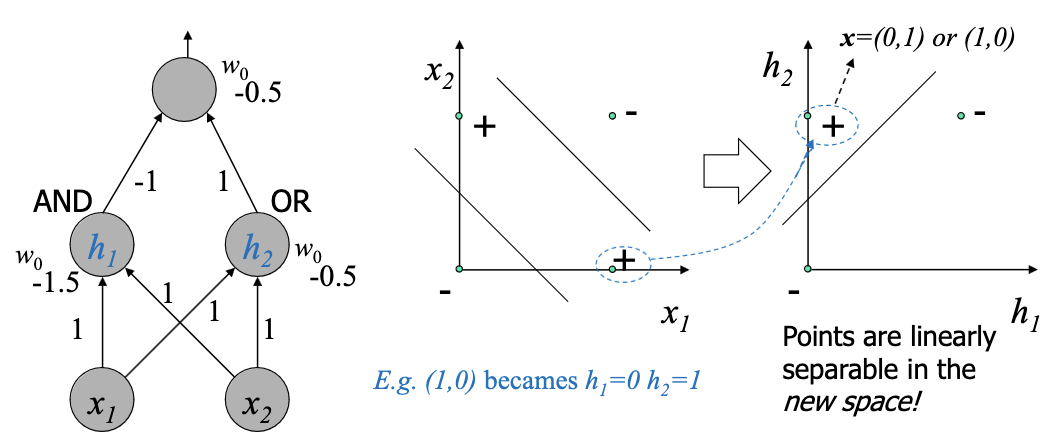
\includegraphics[width=0.5\linewidth]{img/xor perceptron.png}
\end{figure}
This type of composition can be used to perform more complex tasks, extending the network to many layers of abstraction. In NN, this internal representation can be learned.

\section{Learning Algorithms For One Unit Models}

There's two kinds of learning algorithms:
\begin{itemize}
    \item \textbf{Adaline (Adaptive Linear Neuron)}: linear unit during training, can use LMS with either SVD or gradient descent algorithm. This approach an be generalized to multi-level perceptron NNs.

    \item \textbf{Perceptron}: non-linear unit during training, with hard limit on the threshold activation function. Can only be used for classification.
\end{itemize}

\subsection{Perceptron Learning Algorithm}

The goal of the algorithm is to minimize the number of misclassified patterns; so it must find $w$ such that $sign(w^Tx)=d$. This is an on-line algorithm, so one step can be done for each input pattern. The algorithm can be summarized as follows:

\begin{enumerate}
    \item Initialize the weights (either to 0 or a small random value);

    \item Pick a learning rate $\eta$;

    \item For each training pattern $<x,d>$, where $d$ is either $+1$ or $-1$, compute $out = sign(w^Tx)$; if $out = d$, don't change the weights, otherwise modify the weights as:
    \begin{equation*}
        w_{new} = w + \eta d x
    \end{equation*}
    or, in a different form,
    \begin{equation*}
        w_{new} = w + \frac{1}{2} \eta (d-out) x
    \end{equation*}
\end{enumerate}

Looking at the problem from a geometrical point of view, it's as if we modified the weight vector $w$ by summing the vector $\eta d x$, where $d$ indicates the direction of the vector with respect to that $x$: if positive, the addition will move $w$ ``towards'' the point, if negative, it will move it ``away'' from it.

The form $w_{new} = w + \eta d x$ is in the form of Hebbian learning, while $w_{new} = w + \eta (d-out) x = w + \eta \delta x$ is in the form of error-correcting learning.

\subsection{Perceptron Convergence Theorem}

``The perceptron is guaranteed to converge (= classify correctly all input patterns) in a finite number of steps if the problem is linearly separable.'' Note that a regressor using LMS does not guarantee convergence.

Let us assume $(x_i, d_i)$ in the TR set, where $d_i \in \{-1,+1\}$. If the problem is linearly separable, here exists $w^*$, solution, such that

\begin{equation*}
    d_i(w^{*T}x_i) \geq \alpha \, , \quad \alpha=\min_i d_i(w^{*T}x_i), \ \alpha > 0
\end{equation*}
hence

\begin{equation*}
    w^{*T}(d_ix_i) \geq \alpha
\end{equation*}
Let us define $x_i' = (d_ix_i)$; then $w^*$ is a solution iff $w^*$ is a solution of $(x_i', +1)$ (it classifies all as positive).  Assuming $w(0) = 0$ at step 0, $\eta = 1$, and $\beta = \max_i\|x_i\|^2$, after $q$ errors (all false negative):

\begin{equation*}
    w(q) = \sum_{j=1}^q x_{(i_j)} \, ,
\end{equation*}
because $w(q) = w(q-1) + x_{i_q}$ according to the update rule used, where $x_{i_j}$ is the vector containing all misclassified patterns for each step $j$ up until the $q^{th}$. Then, we can define the upper and lower bounds for $\|w(q)\|^2$:

\begin{itemize}
    \item the lower bound is given by:
    \begin{align*}
        &w(q) = x_{i_0} + x_{i_1} + \dots + x_{i_q} \\
        &w^{*T}w(q) = w^{*T}x_{i_0} + w^{*T}x_{i_1} + \dots + w^{*T}x_{i_q} \geq q \alpha \ ,
    \end{align*}
    since $w^*$ is the optimal solution.
    With Cauchy-Swartz, it holds that:
    \begin{equation*}
        \|w^{*T}\|^2\|w(q)\|^2 \geq (w^{*T}w(q))^2 \geq (q \alpha)^2
    \end{equation*}
    so
    \begin{equation*}
        \|w(q)\|^2 \geq (q \alpha)^2 / \|w^*\|^2
    \end{equation*}

    \item the upper bound is given by:
    \begin{equation*}
        \|w(q)\|^2 = \|w(q-1) + x_{i_q}\|^2 = \|w(q-1)\|^2 + 2w(q-1)x_{i_q} + \|x_{i_q}\|^2
    \end{equation*}
    where $w(q-1)x_{i_q} < 0$ since it produces a misclassification; therefore
    \begin{equation*}
        \|w(q)\|^2 \leq \|w(q-1)\|^2 + \|x_{i_q}\|^2
    \end{equation*}
    and, by iteration, since $w(0) = 0$:
    \begin{equation*}
        \|w(q)\|^2 \leq \sum_{j=1}^q \|x_{i_j}\|^2 \leq q \beta
    \end{equation*}
    
\end{itemize}
Putting it all together:

\begin{equation*}
    \dfrac{(q \alpha)^2}{\|w^*\|^2} \leq \|w(q)\|^2 \leq q \beta
\end{equation*}
Therefore:
\begin{equation*}
    q \leq \dfrac{\beta}{\alpha^2 / \|w^*\|^2}.
\end{equation*}


\subsection{Differences Between LMS and Perceptron Learning Algorithm}

They are apparently very similar; they both calculate the new value of $w$ by adding a $\delta$ multiplied by the learning rate $\eta$, along with the input $x$ for the Perceptron Learning Algorithm. The $\delta$ for LMS is calculated as $(d - w^Tx)$, while for perceptron learning algorithm it's $(d - sign(w^Tx))$. However similar they are, there a few important differences:

\begin{itemize}
    \item LMS does not necessarily minimize the number of training examples misclassified by the LTU, since it changes the weights for both misclassified and correctly classified ones;

    \item The perceptron learning algorithm always converges for a linear separable problem to a perfect classifier, while LMS has asymptotic convergence (also for non linearly separable problems);

    \item The perceptron learning algorithm is difficult to extend to a NN, while the LMS can be extended to a NN by using the gradient based approach.
\end{itemize}

\section{Activation Functions}

As seen before, the possible activation functions can be a linear function, a threshold function (perceptron/LTU), or a non-linear function such as the \textbf{sigmoidal logistic function}. The latter is a function that assumes a continuous range of values in the bounded interval $[0,1]$. It has the important property of being a smoothed differentiable function. The slope of the sigmoid function is defined by the parameter $a$. Some common examples of functions are:

\begin{itemize}
    \item \textbf{Logistic function}: $f_{\sigma}(x) = \dfrac{1}{1+e^{-ax}}$ (with output in the range $[0,1]$)

    \item \textbf{tanh function}: $f_{tanh}(\frac{x}{2}) = 2f_{\sigma}(x) - 1$ (with output in the range $[-1,+1]$)

    \item \textbf{Radial basis function}: $f(x) = e^{-ax^2}$

    \item \textbf{Rectified linear unit (ReLU)}:
    $f(x) = \begin{cases}
            0 & x < 0 \\
            x & x \geq 0
            \end{cases}$

    \item \textbf{Softplus function}: $f(x) = ln(1+e^x)$
\end{itemize}

The derivative of the identity function is 1. The derivative of the threshold function is not defined, which is why it's not used in LMS. As for sigmoid functions:

\begin{equation*}
    \dfrac{df_{\sigma}(x)}{dx} = f_{\sigma}(1-f_{\sigma}(x)) 
\end{equation*}

\begin{equation*}
    \dfrac{df_{tanh}(x)}{dx} = 1 - f_{tanh}(x)^2
\end{equation*}

\section{LMS With Sigmoidal Function}

Since the sigmoidal logistic function is differentiable, we can derive a LMS algorithm by computing the gradient of the mean square loss function as for the linear units. The output of a neuron is calculated as:
\begin{equation*}
    out(x) = f_{\sigma}(x^Tw)
\end{equation*}
The objective of the algorithm is to find $w = argmin_w E(w) = \sum_p (d_p - out(x_p))^2 = \sum_p (d_p - f_{\sigma}(x_p^Tw))^2$, so the weights that minimize the residual sum of squares.

The gradient descent algorithm is the same, except it uses the new delta rule: $w_{new} = w + \eta \delta_p x_p$, where $\delta_p = (d_p - out(x_p))f'_{\sigma}$. Additionally, the parameter $a$, the slope of the function $f_{\sigma}$, can affect the step of the gradient descent.

Overall: the max of $f'$ corresponds to net inputs close to 0, while the minimum of $f'$ corresponds to \textbf{saturated cases}, as in where the function $f$ goes to either 0 or 1 asymptotically.

\section{Multi Layer Perceptrons}

A MLP can be seen in two possible ways: either as a network of units, or as a flexible function. As a network, a MLP contains a number of units connected by \textbf{weighted links}. The units are organized in layers: the first layer that loads the input is called the \textbf{input layer}; the layer that produces the final output is called the \textbf{output layer}; all other inbetween layers are called \textbf{hidden layers}. The notation used to refer to networks will be the following:

\begin{itemize}
    \item the index $t$ denotes a generic unit, while $k$ denotes an output unit;

    \item the index $u$ denotes a generic input component;

    \item $x$ is a generic input from an external source (if it's an input vector) or from another unit;

    \item if the pattern $x$ is loaded in the input layer, the notation $o$ can be used for both inputs and hidden layer inputs, so, inside the network, the input to each unit $t$ from any source $u$ is simply denoted as $o_u$.
\end{itemize}
As a flexible function, the MLP can be written as a function in the following form:

\begin{equation*}
    h(x) = f_k(\sum_j w_{kj} f_j (\sum_i w_{ji} f_i(\dots))) \, ,
\end{equation*}
where $f_k$ is a sigmoid activation function.

\subsection{Architecture}

The architecture of a NN defines the topology of the connections between units. A \textbf{feedforward architecture} describes a network that operates as follows. For each input pattern $x$, do:

\begin{enumerate}
    \item load the input in the input layer;
    \item compute the output of all the units in the first hidden layer;
    \item compute the output of all the units in the second hidden layer;
    \item ...
    \item compute the output of all the units in the output layer;
    \item compute the error (delta) at the output level.
\end{enumerate}
A \textbf{recurrent architecture} describes a network with feedback loops, which allow the output of units to go ``back'' in the network towards units in previous layers.

\section{Flexibility of NNs}

The hypothesis space of a NN is the continuous space of all the functions that can be represented by assigning the weight values of the given architecture. Depending on the class of values produced as output, the model can deal with both regression and classification tasks, by using, respectively, a linear function or a sigmoidal one. It can also implement multi-regression and multi-class classifiers by defining multiple output units.

When we consider a NN as a function, so in the form
\begin{equation*}
    h(x) = f_k(\sum_j w_{kj} f_j (\sum_i w_{ji} f_i(\dots))) \, ,
\end{equation*}
each $f_j$ can be seen as computed by an independent unit, or a special kind of $\phi$ of Linear Basis Expansion. Additionally, $h(x)$ is non-linear in the parameters $w$. So, we can reformulate the function as follows:
\begin{equation*}
    h(x) = f_k(\sum_j w_{kj} f_j (\sum_i w_{ji} x_i)) = f(\sum_j w_j \phi_j(x,w))
\end{equation*}
The main difference with LBE is that the $\phi$ are adapted to data by fitting the $w$.

\subsection{Theoretical Grounds}

The universal approximation theorem declares that single hidden-layer network (with logistic activation functions) can approximate (arbitrarily well) every continuous function, given enough units; a MLP network can approximate (arbitrarily well) every input-output mapping (provided enough units in the hidden layers), as well. Note that this theorem does not say which learning algorithm to use, nor the number of units needed.

Two issues arise: how can we learn with a NN?, and, how can we decide what NN architecture to use? The answers to these two questions will be provided later. The expressive power of NN is strongly influenced by two aspects: the number of units and the architecture. More specifically, the number of parameters $w$ (which is proportional to the number of units) influences the network capabilities; additionally, even their value can influence the VC-dim of the network: the lower the weights, the lower the VC-dim.

Another important aspect is the number of layers to use in the network. The universal approximation theorem tells us that 1 layer is sufficient to approximate any function, yet it gives no indication on the number of units to use, which may be incredibly high. So, instead of using only one layer, the network is split into multiple layers, each with a limited number of units.

\section{Backpropagation Learning Algorithm}

The learning algorithm used for NN follows the LMS approach. The goal is to adapt the free parameters $w$ in order to obtain the best approximation of the target function. This is normally done by checking the value of the error (or loss) function calculated on the training set. In the case of NNs, however, this is not as straightforward: the network has multiple units across layers, so the learning algorithm must first decide how much credit to give to the hidden units in causing the error to increase.

The so called \textbf{loading problem} is formulated as follows: given a network and a set of examples, is there a set of weights so that the network will be consistent with the examples? The problem is NP-complete, and while networks can in practice be trained in a reasonable amount of time, an optimal solution in not guaranteed.

The idea behind the backpropagation algorithm solution is to extend the gradient descent approach, so it can be used with MLP networks as well. The things we need are:
\begin{itemize}
    \item differentiable loss;
    \item differentiable activation functions;
    \item a network to follow the information flow.
\end{itemize}
What we want to find is $w$ obtained by computing the gradient of the error function. The advantages of the backpropagation algorithm are:
\begin{itemize}
    \item it's easy because of the compositional form of the model;
    \item it keeps track of the quantities local to each unit;
    \item it's efficient, since it's $O(\#W)$ rather than $O(\#W^2)$
    \item supposedly, the brain's learning ``algorithm'' is a local sub optimal approximation of backpropagation (although this debate remains controversial).
\end{itemize}

\subsection{Issues in Training NNs}

The resulting model is often over-parameterized; additionally, the optimization problem is no longer convex, and is potentially unstable.

Some problems in training NNs involve:
\begin{itemize}
    \item \textbf{Hyperparameters}: starting values, choosing between on-line/batch, learning rate, number of hidden units in the network;

    \item \textbf{Multiple minima}: the loss is no longer a simple convex function, so finding a minimum needs specific techniques;

    \item \textbf{Stopping criteria};

    \item \textbf{Overfitting and regularization};

    \item \textbf{Input scaling/output representation}.
\end{itemize}

\subsubsection{Hyperparameters}

\paragraph{Starting values}

The weights are normally initialized with random values near 0; we want to avoid a completely null weight vector, too high values, or all components equal to each other, since these can hamper training. We can also consider the \textbf{fan-in}, i.e., the number of inputs to a hidden unit: $range * 2 /fan-in$. This should be avoided if the fan-in is too large, or if the unit in question is an output unit, since the $\delta$ would be too close to 0 (since we're using backpropagation, those $\delta$ values would be propagated to previous layers, and cause all others to decrease as well).

There's other heuristics, such as a relatively recent one proposed by \href{https://proceedings.mlr.press/v9/glorot10a/glorot10a.pdf}{Glorot and Bengio}.

\paragraph{On-line or Batch gradient descent}

The batch version of the algorithm calculates all the gradients of each pattern over an epoch, then it updates the weights. The stochastic version instead updates the weights after calculating the gradient on one pattern at a time; it also needs a smaller learning rate $\eta$ compared to the batch version, since a value too high may produce a training that's too ``chaotic''.

In terms of MLP with backpropagation, the way the gradient is calculated is:

\begin{equation*}
    - \dfrac{\partial E(w)}{\partial w_{tu}} = - \sum_{p=1}^l \dfrac{\partial E_p(w)}{\partial w_{tu}} = \sum_{p=1}^l \delta_{p,t} o_{p,u}
\end{equation*}
for the batch version, and:
\begin{equation*}
    - \dfrac{\partial E(w)}{\partial w_{tu}} = \delta_{p,t} o_{p,u}
\end{equation*}
for the on-line version.

The batch version produces a more accurate estimation of the gradient, but the on-line version can help avoid local minima while not being as accurate. Additionally, when using the on-line version, a random shuffling of the patterns should be done before each epoch, in order to avoid any bias in the gradient descending.

A variant of the on-line version is the \textbf{minibatch (MB)}. In this version, the epochs are divided in parts; the gradient is summed up to $mb$ patterns ($mb$ = the size of a part) before updating the weights, instead of updating them after every single calculation. Indeed, the batch an on-line versions can be seen as extreme cases of the minibatch: the first uses a part that's exactly the same size as the dataset, the other uses parts of size = 1. A commonly used value of $mb$ is 100, since it's the ideal partitioning of the dataset that exploits GPU memory parallelism the best.

Basic SGD is generally efficient even with NNs, but depends on the number of training data and the number of epochs. There's other heuristic approaches, such as Quick-prop, in which we go to the minima of the local estimated convex function, or R-prop, which does not use the value of the gradient and instead only its' sign.

Some commonly used approaches are \textbf{second order methods}, which calculate more information about the curvature of the objective function in order to plan a better descent. Some methods include approximation of Newton's methods, and Hessian free approaches (conjugate gradients and quasi-Newton methods). These methods, however, have never replaced gradient descent for NN training, because they are susceptible to saddle points (which grow exponentially in high dimensional spaces); gradient descent, instead, shows how to escape saddle points. The length of the training path with gradient descent may still be high for reasons unrelated to local minima or saddle points, however; the reason is still subject of studies. 

In practice, the main basic approaches are more that enough if applied correctly. After all, this optimization is done on the training set, but our focus should be on validation.

\paragraph{Learning rate}

An higher value of $\eta$ causes the descent to be faster but more unstable; a lower value of $\eta$ causes the descent to be slower but more stable. A way to monitor the behavior of the model (and adjust the learning rate as desired) is to plot the \textbf{learning curve}, which is obtained by plotting the error against the number of epochs. Depending on the value of $\eta$, the curve may have a different appearance.

\begin{figure}[h]
    \centering
    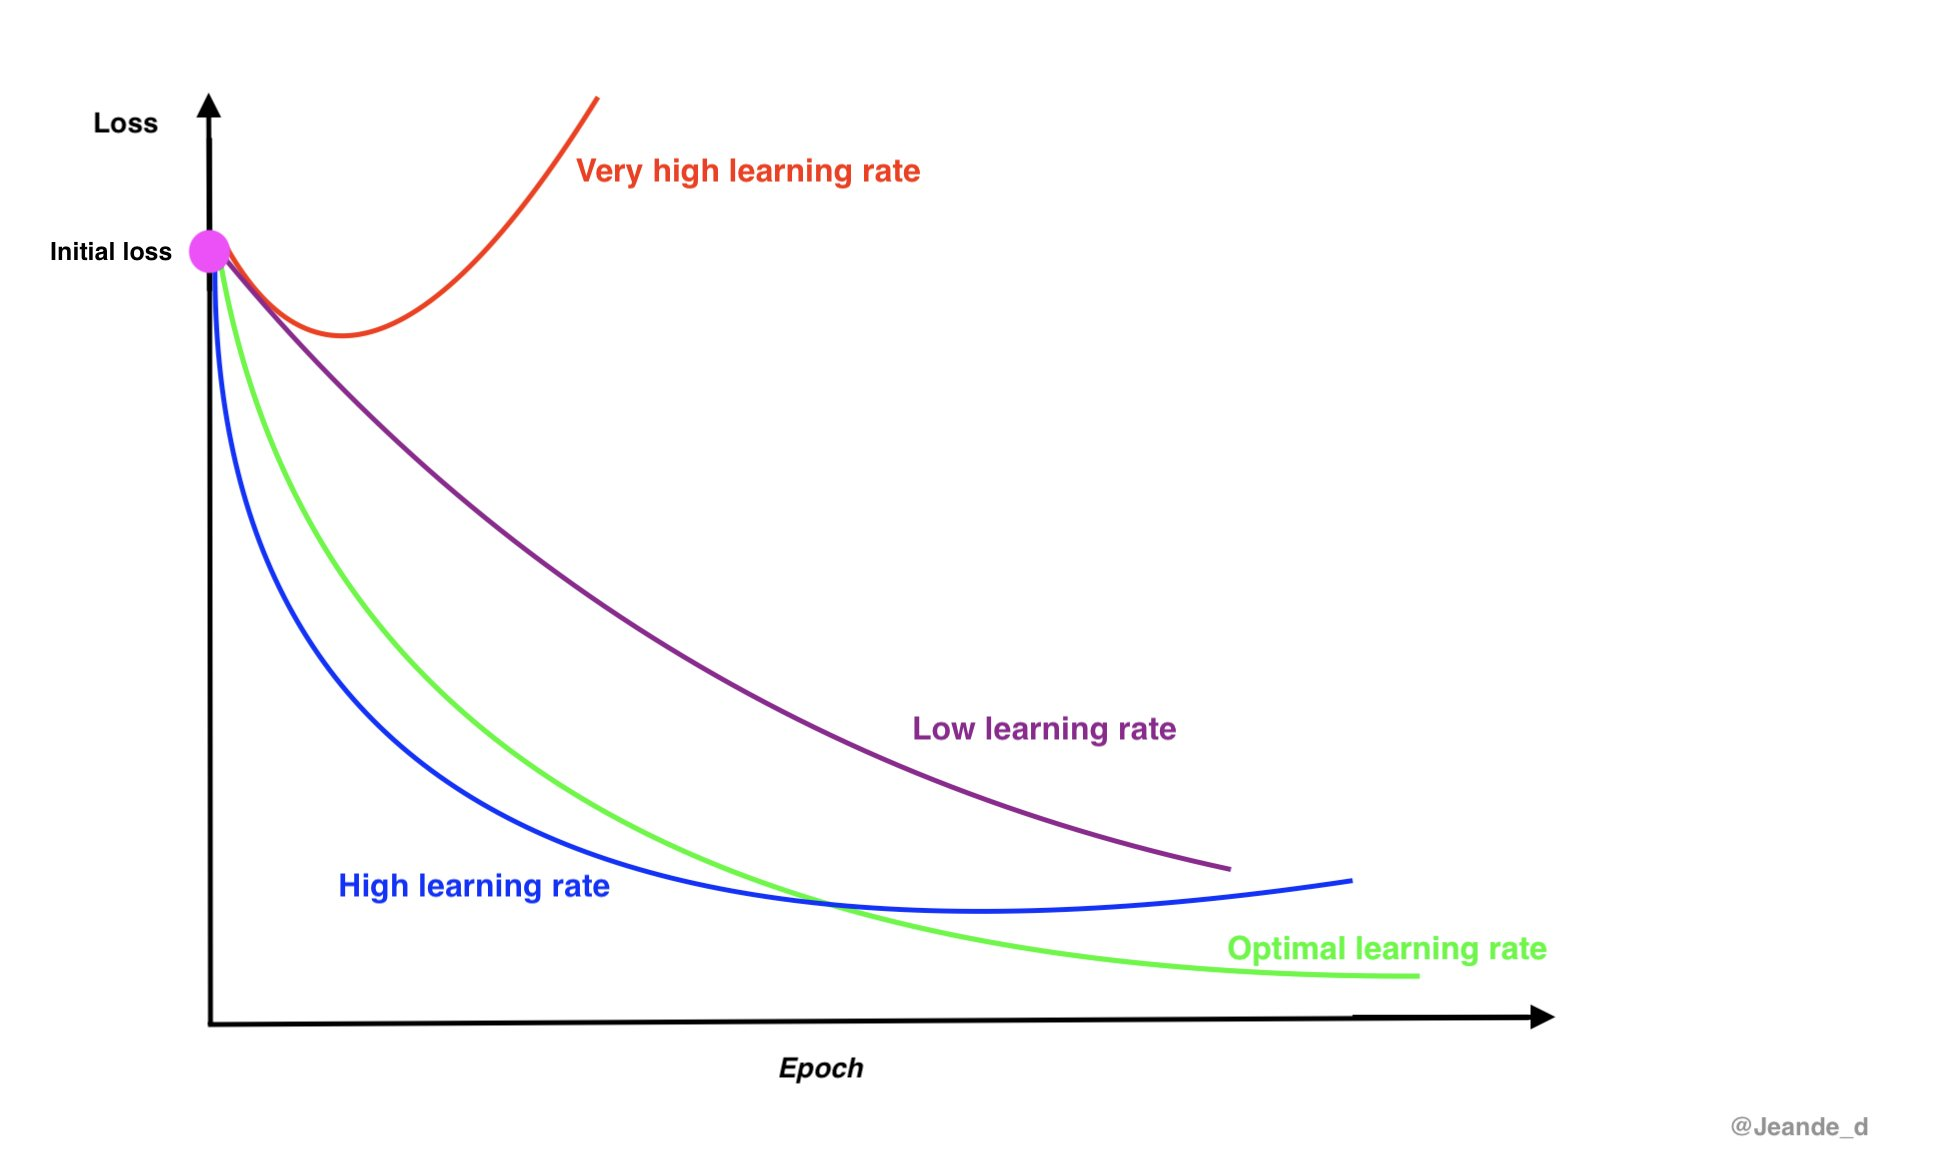
\includegraphics[width=0.5\linewidth]{img/Learning curve and eta.png}
\end{figure}
The green line may appear smooth, but it's actually irregular if we zoom in:
\begin{figure}[h]
    \centering
    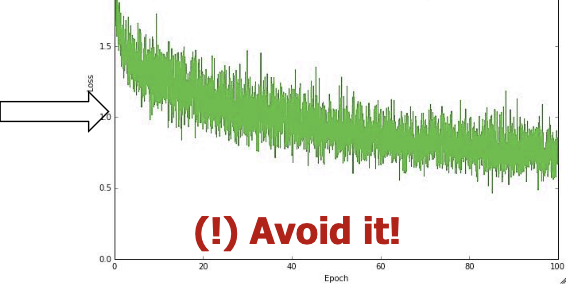
\includegraphics[width=0.5\linewidth]{img/immagine.png}
\end{figure}

In a practical approach, it's useful to consider the mean of the gradients over the epoch, in order to have a uniform approach with respect to the number of input data. When using LMS, dividing by $l$ is equivalent to using $\eta/l$ as our learning rate. As a way to improve the choice of learning rate, the following approaches may be considered:

\begin{itemize}
    \item Using \textbf{momentum}: by adding momentum, $\Delta w$ is now calculated as:
    \begin{equation*}
        \Delta w = - \eta \dfrac{\partial E(w)}{\partial w} + \alpha \Delta w_{old} \, ,
    \end{equation*}
    so we introduce a new term that depends on the previous value of $\Delta w$. $\alpha$ is a value between 0 and 1.

    This is called the ``heavy ball method''. It's faster in plateaus, because the same sign of gradient causes the momentum to increase the delta, and also compensates oscillations in the training, allowing us to use a higher value of $\eta$. It's commonly assumed to help with batch mode more, but can also be used with on-line; in this case, $\Delta w_{old}$ is the $\Delta w_{p-1}$ (as in, of the previous example).

    A variant of momentum is the \textbf{Nesterov momentum}, where the gradient is evaluated after the momentum is applied; so we firs calculate $w = w + \alpha \Delta w_{old}$, the we evaluate the gradient on this new $w$. This variant has been shown to improve the rate of convergence for the batch mode, but not for the stochastic mode.
    
    \item Variable learning rate (start high, then decrease):
    using minibatch, the gradient does not reach 0 even when close to a minimum (as exact gradient can do), hence a fixed learning rate should be avoided. We can linearly decay $\eta$ for each step until iteration $\tau$, using $\alpha = step / \tau$:
    \begin{equation*}
        \eta_s = (1-\alpha)\eta_0 + \alpha \eta_{\tau} 
    \end{equation*}
    and then stop for some iteration, from which we can use a fixed small value of $\eta$. Ideally, the final value of $\eta$ should be $\sim 1\%$ of $\eta_0$, so it takes a few hundred steps to reach it.
    
    \item Adaptive learning rates (changed during training and for each $w$): automatically adapt the learning rate during training, avoiding or reducing the fine tuning phase via hyperparameter selection. Some popular ones include AdaGrad, RMSProp, Adam. Can be combined with momentum.
    
    \item Varying in NNs with many layers (higher for deep layers, or higher for units with few input connections).
\end{itemize}

\paragraph{Number of units}

The number of units controls the complexity of the NN. This choice is in general a model selection issue, so it's selected by a cross-validation. Few units typically lead to underfitting, while too many lead to overfitting, but we can have NNs with many units that don't overfit if regularization is used. We can follow two approaches; either a \textbf{constructive}, incremental, one, in which the learning algorithm decides the (small) starting number of units and then adds more as needed, or a \textbf{pruning} one, where we start with a large network and progressively eliminate weights or units.

A common constructive approach is the \textbf{Cascade Correlation (CC)} learning algorithm. It starts with a minimal network, and adds units until the error is low. It learns both the network weights and topology.

\begin{algorithm}
\caption{Cascade Correlation algorithm.}
\begin{algorithmic}[1]
    \State Start with N0, a network with no hidden units, train it and calculate the error.

    \If{N0 does not solve the problem}
        \State Set i = 1.
        \Repeat 
            \State Create a new unit, and add to the network (creating Ni).
            
            \State Train the unit so that the correlation between the output of the unit and residual error of network Ni-1 is maximized.

            \State Freeze the weights of the unit, and retrain all other units.
            
            \State Calculate error of the new network.
            \State Increase i by 1.
        \Until{Error is $\leq$ a given threshold.}
    \EndIf
\end{algorithmic}
\end{algorithm}
Specifically, this algorithm works by interleaving the minimization of the error function with the maximization of the correlation, which is the covariance of the output of the new unit with the residual error. The role of hidden units is to reduce the residual output error.

\subsubsection{Multiple Minima}

Loss in no longer convex. The function may have multiple minima, as well as maxima. The final result depends a lot on the starting weight values. Ideally, we should try a number of random starting configurations (trials), and then take the mean result (as in, the mean of errors) and check the variance in order to evaluate the model. Then, we can either pick the solution that produces the lowest/median validation error, or we can consider the mean of the outputs.

It's worth noting that finding a local minima with too high error that stops training is not a big issue, since we can always check the final training error (and restart if needed). In general, we don't need to find the global minimum, a ``good'' local minima is sufficient. This is because the minimum we find is of $R_{emp}$, not $R$ (which is what we want to approximate). Also, instead of finding a point corresponding to the null gradient, we may want to stop at a point that has sufficiently small gradient.

Another aspects to consider is that the NN builds a variable size hypothesis space, and tends to increase the VC-dim during training. As the VC-dim increases, the $R_{emp}$ decreases towards the global minimum, but we'll likely incur into overfitting, so stopping before we find the minimum might actually produce a better approximation of the target function.

\subsubsection{Stopping Criteria}

The basic stopping criteria is to check the error (mean or max error $ E$), however, we may not always have enough information to set a tolerance threshold for the error. We may want to use an internal criterion: we stop if the improvement of the error (e.g., less than 0.1\%), or the changes to the weights (e.g. norm of gradient $ < \eta$) are negligible.

We must not stop at an arbitrary number of steps; if it's too small, then it may be too early and cause underfitting, while if it is too large, we may incur into overfitting. Also, if we use K-Fold cross validation, the number of ideal steps for each fold may vary: how do we choose it for the final model, trained over all data? We can consider the number of epochs as a hyperparameter, and select its value as the mean across the folds; however, changing the data size at the end, adding all the records of validation and test set, the stop point may be different, leading to underfitting.

\subsubsection{Overfitting and Regularization}

As said before, we typically don't want the global minimizer of $R_{emp}$, since it would be an overfitting solution. The control of complexity requires some form of regularization (as seen for LBE). This can be achieved by introducing a penalty term, or indirectly by early stopping. Another important step is to perform cross-validation on empirical data to find the best trade-off.

In NNs, learning normally starts by setting the weights to small, random values, and the VC-dim is low. As optimization proceeds, hidden units tend to saturate, increasing the number of free parameters, hence increasing the VC-dim. So, how do we choose when to stop this optimization?

\begin{itemize}
    \item \textbf{Early stopping}: using a validation set to determine when to stop. We ideally want to consider multiple epochs to estimate the error. Since the effective number of parameters grows during the course of training, stopping means limiting the complexity.

    \item \textbf{Regularization}: we can use a regularization related to Tikhonov theory, applied to the loss; a penalty term is added, such that the loss will be calculated as:

    \begin{equation*}
        Loss(w) = \sum_p (d_p - o(x_p))^2 + \lambda\|w\|^2
    \end{equation*}
    This is a form of weight decay, since the new values of the weights during gradient descent will be calculated by adding the term $- \lambda w$, which causes it to decrease even when $\Delta w$ is 0. The regularization parameter $\lambda$ is generally a low value, and is selected in the model selection phase.

    \item \textbf{Pruning methods}: will see later.
\end{itemize}

Remember that, when using regularization, the loss is used during model training, while the error (or risk) for the ``data term'' is used during model evaluation, since it only measures how different the output of the hypothesis is from the correct label. A common misconception is that regularization helps convergence stability, but it does not. It only controls the complexity.

Also, early stopping and regularization can be used together. The difference is that early stopping is an \textbf{empirical approach}, that requires a VL set to decide a stopping point, while regularization is a \textbf{principled approach}, and allows the VL curve to follow the TR curve.

Note, also, that the bias $w_0$ is often omitted from the regularizer, since its inclusion causes the results to not be independent from target shift or scaling. If it's included, it has its own regularization term.

\subsubsection{Putting Momentum and Weight Decay Together}

By putting the two together, the $\Delta w$ can be calculated as:

\begin{equation*}
    \Delta w = -\eta \dfrac{\partial Loss(w)}{\partial w_{tu}} + \alpha \Delta w_{old_{tu}} \doteq \eta \delta_t o_u - \lambda w_{tu} + \alpha \Delta w_{old_{tu}}
\end{equation*}
Here, the index $p$ is omitted and we consider the Loss as the sum of Error + Penalty and using $\eta$ only for the Error term. This form, where $\Delta w$ includes $\lambda$, $\eta$ and $\alpha$, is often used by major tools/libraries for NNs. However, we can define a form that keeps the hyperparameters separated, b y writing:

\begin{equation*}
    \Delta w = \eta \delta_t o_u + \alpha \Delta w_{old_{tu}} \, ,
\end{equation*}

\begin{equation*}
    w_{new_{tu}} = w_{tu} + \Delta w_{tu} - \lambda w_{tu} 
\end{equation*}
In this form, eta and alpha are independent.

\subsubsection{Input Scaling/Output Representation}

Preprocessing of the data can have a large effect on the result of training. Data should be normalized via either standardization (each feature is modified so that mean is 0 and standard deviation is 1), or rescaling (the range of values is restricted to [0,1]).

For regression, there's one or more output linear units; for classification, there's either a singular binary output unit, or there's multiple binary units. In the latter case, we can use a sigmoid to choose the threshold to assign the class, a rejection zone, or 1-to-K encoding to choose the ``winner'' class. Often, the symmetric logistic function learns faster. To avoid asymptotic convergence, 0.9 and 0.1 can be used instead of 1 an 0 as a label value (for the logistic function, for the tanh function -0.9 is used instead of -1). In any case, the target range must be in the output range of units. If targets are 0/1, it's common to use the Softmax function:

\begin{equation*}
    o_k(x) = \dfrac{e^{(-net_k)}}{\sum_{j=1}^Ke^{(-net_j)}}
\end{equation*}
We can also use an alternative error/cost function, where we minimize the cross entropy:

\begin{equation*}
   E(w) = - \sum_{i \in TR} \{ d_i \log (out(x_i)) + (1-d_i) \log(1-out(x_i)) \}
\end{equation*}

\section{When To Consider NNs}

\begin{itemize}
    \item The input is high dimensional discrete or real-valued, both for regression and classification tasks;

    \item The dataset possibly contains noise;

    \item The form of the target function is unknown;

    \item Human readability of the output is not critical;

    \item Training time is not critical;
    
    \item The computation of the output itself has to be fast.
\end{itemize}
\chapter{Validation and SLT}

When a model is being trained, we're looking at the best solution, i.e., the best balancing between fitting of the training data and model complexity, as not to incur into over- or underfitting. Obviously, the training set cannot be used to estimate the test error, as low training error leads to overfitting.

Assume we have only one hyperparameter $\theta$ that varies the model complexity, and we want to find the ``best''value of it. The estimation of the error can be approximated, either analytically (e.g., AIC, BIC for linear models, Minimum Description Lenght, Structural Risk Minimization and so on), or by resampling, so via \textbf{cross-validation} or bootstrap.

Remember the distinction between model selection and model assessment:
\begin{itemize}
    \item \textbf{Model selection} estimates the performance of different models in order to select the one the generalizes the best; this phase returns a model;

    \item \textbf{Model assessment}: having chosen a final model, it estimates its prediction error/risk by using unseen data (the test set), and returns an estimation value.
\end{itemize}

The gold rule is to keep separation between the goals, and for each goal to use a different set: one for training, one for validation, and one for testing.

Let's see an example. Assume we have 20-30 examples, with 1000 input variables. The target (random) is 0/1. We select a model with a single input variable that guesses 100\% on any splitting of the data in TR/VL/TS. This means that we produced a model that apparently always finds the correct output... or does it? In reality, the true error estimation is 50\%; this is because the chosen variable just so happens to match the target values. But in a real application, the model is basically coin guessing the output. In summary, the error estimated on the training set (and validation set) is not a good estimation of the generalization error; we need a new set of unseen data to do so.

\begin{figure}[h]
    \centering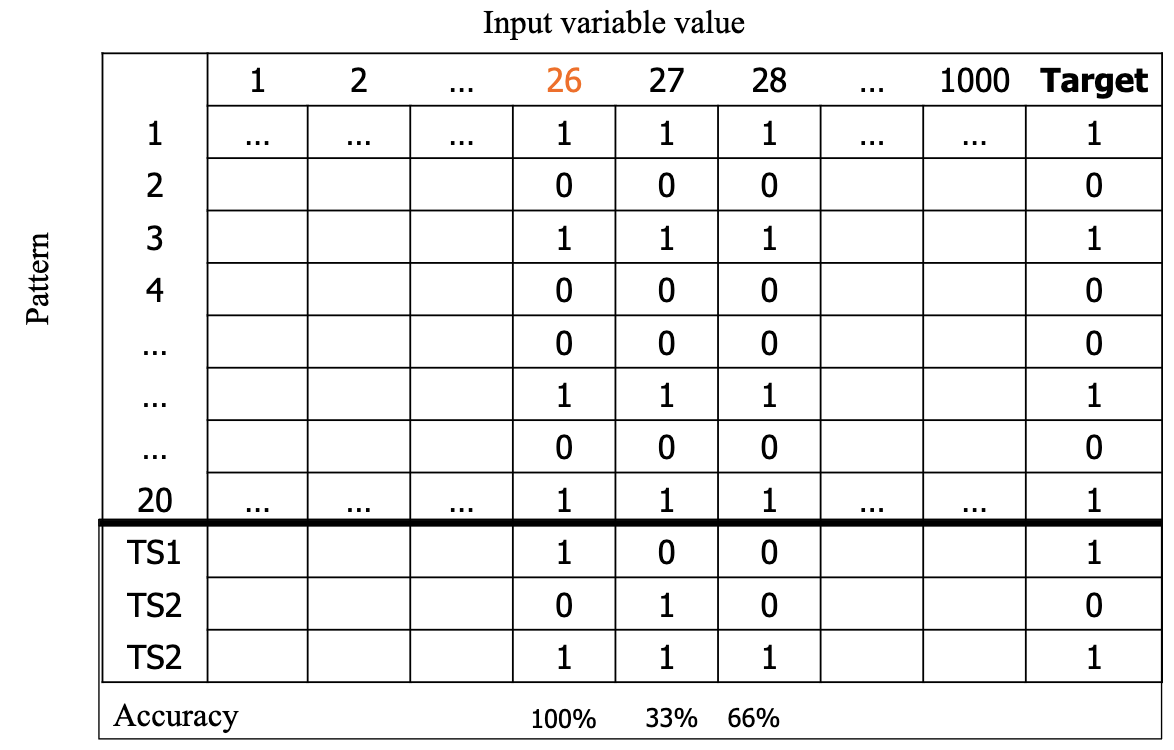
\includegraphics[width=0.5\linewidth]{img/table_counterex.png}
\end{figure}

\section{Grid Search}

Since hyperparamters are not learned by the learning algorithm, it's our task to find the best values for them. Choosing them is done by calculating the error on the validation set (VL). 

One way to search for hyperparameter values is to perform a grid search; candidates are generated from a grid of parameter values and tested on the validation set. This technique can have an high cost, since the total number of candidates is equal to $n^m$, where $n$ is the number of values in the range and $m$ is the number o f hyperparameters. For this reason, grid search is typically used to fix some values in preliminary phases.

Additionally, we can perform two or more levels of nested grid search. First we apply a coarse search to a table with the combinations of all possible values set at intervals (e.g., growing exponentially) in order to find the best interval. Then we apply a second grid search by considering only the values withing that interval, and we can repeat the grid search until we perform a search fine enough for our needs.

There are alternatives to grid search, such as random search, automatized search, and many more offered by popular libraries.

\section{K-fold Cross Validation}

The most basic way of setting up data for model selection and model assessment is to split all of our data into three partitions (hold out cross validation). One of them will be the training set, one the validation set, and one the test set. However, it can be difficult to decide how to perform this split; it can depend on the complexity of the model, and signal-to-noise ratio. Also, how can we split the data so that each part is sufficiently sized? And can we avoid to perform a split that influences the results?

K-fold cross validation is another technique that can be used to split the data. Typically, the data is split into TR set and TS set. Then, k-fold cross validation is used over the TR set to obtain new ripartitions of the data to form different TR sets and VL sets. After finding the best hyperparameters, the model is retrained on the whole original TR set, and is assessed on the external TS set. Again, if the estimation is good enough, the model can be retrained on the test set data as well to produce the final model.

K-fold cross validation can still present some problems. It may be influenced by biases in the sample of data used. Cross validation can be repeated, by performing different splits with different random sampling; the estimation can be obtained by averaging the results. Another issue is having a sample too small to accurately represent the general population.

\section{Statistical Learning Theory}

\subsection{Vapnik-Cervonenkis Dimension}

The VC-dim (Vapnik-Cervonenkis dimension) is a measure of the complexty of a class of hypotheses $H$. It does not depend on the actual cardinality of the space, but on the number of distinct instances that can be completely discriminated (i.e., without error) using $H$.

Given $X$ an input space of size $N$, and $H$ the hypothesis space, assume a binary classification task; there are $2^N$ possible \textbf{dichotomies} (i.e., partitions of the $N$ points either -1 or 1). A particular dichotomy is \textbf{represented} in $H$ if there exists an hypothesisi $h$ in $H$ that realizes the dichotomy.

\BoxDef{Shattering}{
The hypothesis space $H$ \textbf{shatters} $X$ iff $H$ can represent all the possible dichotomies on $X$.
}

\BoxDef{VC-dimension}{
The VC-dimension of a class of functions H is the maximum cardinality of a configuration of points in $X$ that can be shattered by $H$.
}

If $VC(H) = p$, it means that there's at least an hypothesis in $H$ that shatters a configuration of size $p$, but cannot shatter any configuration of size $p+1$. If arbitrarily large (but finite) sets of $X$ can be shattered by $H$, then $VC-dim$ is infinite. Note that there needs to be just one configuration of $p$ points that is shattered by an $h$; $h$ does not need to shatter all configurations of size $p$.

To make the concept clearer, consider an hypothesis space $H$ that is a set of lines ($h(x) = sign(wx + w_0) , \, x \in IR^2$). Each dichotomy is a different labeling of points as -1 or 1. This hypothesis space shatters some configurations of 3 points, such as the one shown in the figure below:

\begin{figure}[h]
    \centering
    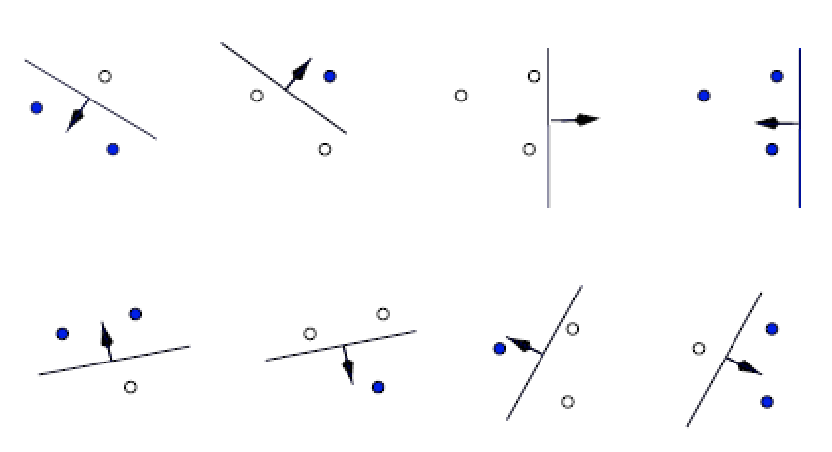
\includegraphics[width=0.5\linewidth]{img/shattering_1.png} 
\end{figure}

but cannot shatter this one:

\begin{figure}[h]
    \centering
    
\includegraphics[width=0.5\linewidth]{img/Shattering_2.png}
\end{figure}

Still, its VC-dim is at least 3, since it can shatter at least the configuration on top. If we consider any configuration of 4 points, a single line cannot always separate them. This means that for any configuration of 4 points, there's at least a dichotomy that is not linearly separable, therefore the VC-dim is less than 4. In general, the VC-dim of a class of linear hyperplanes (LTU) in an $n$-dimensional space is $n+1$.

VC-dim is not the number of free parameters, although it is related. There exists models with only one free parameter and infinite VC-dim, such as K-NN. However, for many reasonable hypthesis classes the VC-dimension is linear in the number of free parameters of the model.

Once we determine the VC-dim, we can then estimate the risk by defining an upper bound:

\begin{equation*}
    R[h] \leq R_{emp}[h] + \epsilon (VC,N,\delta)
\end{equation*}

The function $\epsilon()$ can be calculated in different ways depending on the task, class of functions, etc. This bound gives us a way to estimate the generalization error based only on training error and VC-dimensionality of $H$.

\subsection{Structural Risk Minimization}

SRM uses the VC-dimension as a control parameter to realize the best estimation of the generalization bound. Assume a nested structure of $n$ models/hypotheses space, such that: 

\begin{gather*}
    H_1 \subseteq H_2 \subseteq \dots \subseteq H_n \\
    VC(H_1) \leq VC(H_2) \leq \dots \leq VC(H_n)
\end{gather*}

An example could be a nested structure of neural networks, where each $H_i$ corresponds to a network containing a different number of units; another could be polynomials with increasing degree.

The more the VC-dim increases, the more the VC-confidence and therefore the bound increase as well. The goal of SRM is to find the model corresponding to the trade-off on the bound between VC-dim and VC-conf.

Once this bound has been determined, can it be used as an estimate of prediction errors? Yes, but rarely. It can be useful during model selection, but it's an overly pessimistic estimate for model assessment.
\chapter{Support Vector Machines}

Support Vector Machines (SVMs) are a type of model used for both classification and regression. They used to be the most popular approach for supervised learning when there's little to no domain knowledge for the data, but they've been mostly replaced by neural networks and random forests.

\section{Hard Margin SVM}

Assume a classification task. Given a training set $TR = <x_i,d_i>, \, i=1 \dots N$, we want to find an hyperplane of equation $w^T x + b = 0$ to separate the examples; specifically, we want:

\begin{gather*}
    w^T x_i + b \geq 0 \text{ for } d_i = +1 \\
    w^T x_i + b < 0 \text{ for } d_i = -1
\end{gather*}

$g(x) = w^T x + b$ is called the \textbf{discriminant function}, and $h(x) = sign(g(x))$ is the hypothesis. Note that here the bias is referred to as $b$ instead of $w_0$. To find the hyperplane that separates all the points, instead of simply minimizing the empirical risk, the SVM minimizes the expected generalization error by finding the separator that is farthest away from all the examples in the dataset. It also establishes a margin ($\rho$) around it, whose width is exactly twice the distance between the hyperplane and the closest data point(s). The optimal hyperplane is the one that maximizes this margin $\rho$: $w_o^Txv + b_o = 0$, where $\rho = 2 / \|w_o\|$.

The two terms $w$ and $b$ can be rescaled so that the closest points to the separating hyperplane satisfy $\|g(x)\| = 1$, so we can write:

\begin{gather*}
    w^T x_i + b \geq 1 \text{ for } d_i = +1 \\
    w^T x_i + b < -1 \text{ for } d_i = -1 \, ,
\end{gather*}
or, in a compact form,
\begin{gather*}
    d_i(w^T x_i + b) \geq 1 \, .
\end{gather*}

Any $x_i$ that satisfies this equation is called a \textbf{support vector}, and is referred to as $x^{(s)}$. Let's denote the distance between the optimal hyperplane and a point $x$ as $r$, such that $x = x_p + r\frac{w_o}{\|w_o\|}$ (where $x_p$ is a point on the hyperplane). Evaluating $g(x)$ we obtain:

\begin{align*}
    g(x) = g(x_p + r\dfrac{w_o}{\|w_o\|}) = \\
    = w_o^Tx_p + b_o + w_o^T r \dfrac{w_o}{\|w_o\|} = \\
    = g(x_p) + w_o^T r \dfrac{w_o}{\|w_o\|} = \\
    = 0 + r \dfrac{\|w_o\|^2}{\|w_o\|} = r \|w_o\| \, ,
\end{align*}
thus, $r = \dfrac{g(x)}{\|w_o\|}$.

Consider the distance between the hyperplane and a positive support vector $x^{(s)}$, then $r$ is calculated as:

\begin{equation*}
    r = \dfrac{g(x^{(s)})}{\|w_o\|} = \dfrac{1}{\|w_o\|} = \dfrac{\rho}{2} \, ,
\end{equation*}
therefore, $\rho = \dfrac{2}{\|w_o\|}$.

\subsection{Primal Problem}

The optimum hyperplane will maximize $\rho$ and minimize $\|w\|$. One approach to find it is to perform a gradient descent to find the $w$ and $b$ that minimize/maximizes them, but there's another approach, that is solving a \textbf{quadratic optimization problem}.

\BoxDef{Quadratic optimization problem (primal form)}{
Given the training examples $TR = < x_i,d_i >$, find the optimal values of $w$ and $b$ which minimize
\begin{equation*}
    \Psi (w) = \dfrac{1}{2}w^T w
\end{equation*}
satisfying the constraints
\begin{equation*}
    d_i(w^T x_i + b) \geq 1 \, .
\end{equation*}
}
The objective function $\Psi (w)$ is quadratic and convex in $w$. The constraints are linear in $w$, and solving the problem scales with the size of the input space $m$.

To solve this problem, the \textbf{Lagrangian multipliers method} is used. The Lagrangian function corresponding to the quadratic optimization problem is constructed:
\begin{equation*}
    J(w,b,\alpha) = \dfrac{1}{2}w^T w - \sum_{i=1}^N \alpha_i(d_i(w^T x_i + b) - 1) \, ,
\end{equation*}
where $\alpha_i \geq 0$ are the \textbf{Lagrangian multipliers}. Each term in the sum corresponds to a constraint of the primal problem; $J$ must be minimized with respect to $w$ and $b$ and maximized with respect to $\alpha$. The solution will correspond to a saddle point of $J$.

If we minimize $J$ with respect to $w$, then:
\begin{gather*}
    \dfrac{\partial J}{\partial w} = \dfrac{2}{2} w - \sum_{i=1}^N \alpha_i(d_i(1*x_i + 0) + 0) = \\
    = w - \sum_{i=1}^N \alpha_i(d_i(x_i)) = 0
\end{gather*}
so
\begin{equation*}
    w = \sum_{i=1}^N \alpha_i(d_i(x_i)) \, .
\end{equation*}
Thus the optimal hyperplane is expressed as:
\begin{gather*}
    g(x) = w_o^T x + b_o = 0 \\
    \iff \\
    \sum_{i=1}^N \alpha_{o,i} d_i x_i^T x + b_o = 0 \, .
\end{gather*}
If instead we minimize it with respect to $b$:
\begin{gather*}
    \dfrac{\partial J}{\partial b} = 0 - \sum_{i=1}^N \alpha_i d_i = 0 \, .
\end{gather*}
These can be substituted in $J$ to study the dual form of the problem.

From the \textbf{Kuhn-Tucker Conditions}, it follows that
\begin{equation*}
    \alpha_i (d_i (w^T x_i + b) - 1) = 0 \, , \forall i = 1, \dots , N
\end{equation*}
in the saddle point of $J$. If $\alpha_i > 0$, then $(d_i (w^T x_i + b) = 1$, and $x_i$ is a support vector. If $x_i$ is not a support vector, then $\alpha_i = 0$. Hence we can restrict the computation to $N_s : w_o = \sum_{i=1}^{N_s} \alpha_{o,i} d_i x_i$. The hyperplane depends only on support vectors.

\subsection{Dual Problem}

To obtain the Lagrangian multipliers $\alpha_i$, we solve the problem in its dual form:

\BoxDef{Quadratic optimization problem (dual form)}{
Given the training examples $TR = < x_i,d_i >$, find the optimal values of $\alpha_i$ which maximize
\begin{equation*}
    Q(\alpha) = \sum_{i=1}^N \alpha_i - \dfrac{1}{2} \sum_{i=1}^N \sum_{j=1}^N \alpha_i \alpha_j d_i d_j x_i^T x_j
\end{equation*}
satisfying the constraints
\begin{gather*}
    \alpha_i \geq 0 \, , \forall i = 1, \dots , N \, ,\\
    \sum_{i=1}^N \alpha_i d_i = 0 \, .
\end{gather*}
}
The value of $\alpha_i$ can be found by solving the quadratic programming (QP) problem, or by more recent and efficient approaches (such as sequential minimal optimization (SMO)). Solving this problem scales with the number of training examples, less with the dimensionality. To find $w_o$ and $b_o$, we proceed as follows:
\begin{gather*}
    w_o = \sum_{i=1}^N \alpha_{o,i} d_i x_i \\
    b_o = 1 - w_o^T x^{(s)} = 1 - \sum_{i=1}^N \alpha_{o,i} d_i x_i^T x^{(s)} \, .
\end{gather*}
How do we use all of this? We don't actually need to explicitly know $w_o$. All we need are calculating the Lagrangian multipliers by solving the dual problem, and then calculating $b_o$. So, given the input pattern $x$, we compute $g(x) = \sum_{i=1}^N \alpha_{o,i} d_i x_i^T x + b_o$, and classify it as $h(x) = sign(g(x))$. Minimizing the norm of $w$ is equivalent to minimizing the VC-dim and VC-confidence of the model.

\BoxDef{Theorem - Vapnik}{
Let $D$ be the diameter of the smallest ball around the data points $x_1 , \dots , x_N$. For the class of separating hyperplanes described by the equation $w^T x + b = 0$, the upper bound to the VC-dim is
\begin{equation*}
    VC \leq min(\lceil \dfrac{D^2}{\rho^2} \rceil, m_0) + 1 \,,
\end{equation*}
where $m_0$ indicates the dimensionality of the input space.
}
Since $D^2 / \rho^2 = Radios^2 \|w\|^2$, VC can be less than $m_0 + 1$ computed for general hyperplanes by constraining the search to the ``regularized'' one with maximum margin.

This approach of finding optimal separating hyperplane maximizing the margin also provides:
\begin{itemize}
    \item An unique solution with zero errors for the binary classifier;
    \item An automatized approach to Structural Risk Minimization that minimizes the VC-confidence without having to deal with hyperparameters;
    \item The use of a solver in the class of constrained quadratic programming (instead of gradient descent) with a nice dual form;
    \item A solution focused on a selection of training data points: the support vectors.
\end{itemize}
But what about noisy or non linearly separable data?

\section{Soft Margin SVM}

In realistic datasets, the training set is not going to be perfect. It will contain noisy points and outliers that make the problem not linearly separable. The solution is to find a separator with a soft margin, that is, a margin that allows some errors within it. Because the margin can allow points to fall inside of it, the support vectors are no longer going to be the closest points to the margin.

We introduce what are called \textbf{slack variables}, which are non negative scalar variables:

\begin{gather*}
    \xi_i \geq 0 \, , \forall i = 1, \dots , N \\
    d_i(w^T x_i + b) \geq 1 - \xi_i \, , \forall i = 1, \dots , N
\end{gather*}
If $x^{(s)}$ is a support vector, it will satisfy the equation:
\begin{equation*}
    d_i(w^T x^{(s)} + b) = 1 - \xi_i 
\end{equation*}
Here, Vapnik's theorem does not hold anymore. The problem can be then rewritten to admit points in the margin.

\BoxDef{Quadratic optimization problem with Soft Margin (primal form)}{
Given the training examples $TR = < x_i,d_i >$, find the optimal values of $w$ and $b$ which minimize
\begin{equation*}
    \Psi(w, \xi) = \dfrac{1}{2}w^T w + C \sum_{i=1}^N \xi_i
\end{equation*}
satisfying the constraints
\begin{gather*}
    d_i (w^T x_i + b) \geq 1 - \xi_i \, , \forall i = 1, \dots N \\
    \xi_i \geq 0 \,, \forall i = 1, \dots N
\end{gather*}
}
The term $C$ is a user-defined regularization hyperparameter; so this version of SVM is no longer ``automatic'' like hard margin SVM was. $C$ is found as the trade-off between empirical risk minimization and capacity term (VC-confidence). If $C$ is too low, we allow many training errors, leading to underfitting. If $C$ is too high, we don't let any training error, leading to overfitting.

\BoxDef{Quadratic optimization problem with Soft Margin (dual form)}{
Given the training examples $TR = < x_i,d_i >$, find the optimal values of $\alpha_i$ which maximize
\begin{equation*}
    Q(\alpha) = \sum_{i=1}^N \alpha_i - \dfrac{1}{2}\sum_{i=1}^N \sum_{j=1}^N \alpha_i \alpha_j d_i d_j x_i^T x_j
\end{equation*}
satisfying the constraints
\begin{gather*}
    0 \leq \alpha_i \leq C \, , \forall i = 1, \dots , N \\
    \sum_{i=1}^N \alpha_i d_i = 0
\end{gather*}
}
The Kuhn-Tucker conditions can be redefined as:
\begin{gather*}
    \alpha_i (d_i (w^T x_i + b) + \xi_i - 1) = 0 \, , \forall i = 1, \dots , N \\
    \mu_i \xi_i = 0 \,, \forall i = 1, \dots , N \, ,
\end{gather*}
where $\mu_i$ are Lagrange multipliers introduced to enforce non-negativity of the slack variables in the primal function. If $0 < \alpha_i < C$, then $\xi_i = 0$. If $\alpha = C$, then $\xi_i \geq 0$. To solve the problem, we again solve the dual problem with respect to $\alpha_i$, and calculate $w_o$ and $b_o$ exactly as before.

\section{Mapping To a High-dimensional Space}

\href{https://en.wikipedia.org/wiki/Cover%27s_theorem#The_Theorem}{If the TR set represents a non-linearly separable problem, the data points can be mapped from the input space to a high-dimensional \textbf{feature space}, where they are linearly separable}. The approach we follow is analogous to the LBE for linear models. We define some function $\phi : \mathbb{R}^{m_0}\xrightarrow{} \mathbb{R}^{m_1}$. Finding this function, however, is not always easy, unless we have some prior knowledge allowing us to select the proper feature space. Also, using high dimensional feature spaces can lead to overfitting.

Given this function, we map all points to the new feature space: $x \mapsto \phi(x)$. The problem is formulated as before, with a new training set $TR = < \phi(x_i),d_i >$, and a new hyperplane $g(x) = w^T \phi(x) + b = 0$. The notation used here incorporates the bias in the weight vector, with $w_0 = b$ and $\phi_0(x) = 1$:
\begin{equation*}
    \phi(x) = (\phi_0(x) = 1, \phi_1(x), \dots , \phi_{m_1}(x))^T
\end{equation*}
The weight vector is now a linear combination of the feature vectors:
\begin{equation*}
    w = \sum_{i=1}^N \alpha_i d_i \phi(x_i)
\end{equation*}
and the hyperplane equation can be written as:
\begin{equation*}
    g(x) = \sum_{i=1}^N \alpha_i d_i \phi^T (x_i) \phi(x) = 0
\end{equation*}
Evaluating $\phi(x)$ may be intractable. Fortunately, under certain conditions we do not need to evaluate it directly, or even know the feature space itself. This is possible with a so-called \textbf{kernel trick}, i.e. by using a function $k$ to directly compute the dot products $\phi^T (x_i) \phi(x)$ in the feature space:
\begin{equation*}
    k : \mathbb{R}^{m_0} \times \mathbb{R}^{m_0} \xrightarrow{} \mathbb{R}
\end{equation*}
This function is known as the \textbf{inner product kernel function}. It's also a symmetric function, so $k(x_i, x) = k(x, x_i)$. Consider the function $\phi(x) = \phi((x_1, x_2)^T) = (x_1^2, \sqrt{2}x_1x_2, x_2^2)^T$. Given $x = (x_1, x_2)^T$ and $y=(y_1,y_2)^T$ in $\mathbb{R}^2$, we compute $\phi^T(x)\phi(y)$ in this 
\begin{gather*}
    \phi^T(x)\phi(y) = (x_1^2, \sqrt{2}x_1x_2, x_2^2) (y_1^2, \sqrt{2}y_1x_2, y_2^2)^T = \\
    x_1^2y_1^2 + 2x_1y_1x_2y_2 + x_2^2y_2^2 = (x_1y_1 + x_2y_2)^2 = \\
    ((x_1,x_2)(y_1,y_2)^T)^2 = (x^Ty)^2 = k(x,y)
\end{gather*}
We can arrange the dot products in the feature space between the img of the input training patterns in a $N$ by $N$ matrix, called \textbf{kernel matrix}:
\begin{equation*}
    K = \begin{pmatrix}
        k(x_1,x_1) & \dots & k(x_1, x_N) \\
        k(x_2,x_1) & \dots & k(x_2, x_N) \\
        \vdots & & \vdots \\
        k(x_N,x_1) & \dots & k(x_N, x_N) \\
        \end{pmatrix} \,, \,
        K = \{k(x_i, x_j)\}_{(i,j)=1)}^N
\end{equation*}
The kernel matrix is symmetrical, as the inner product kernel is symmetrical. Not every kernel function computes the inner product in a feature space; this property holds only for kernels gaining positive semi-definite kernel matrices. This is related to the matrix having non negative Eigenvalues.

Given $k_1$ and $k_2$ both kernels over $\mathbb{R}^{m_0} \times \mathbb{R}^{m_0}$. The following are also kernel functions:
\begin{itemize}
    \item $k_1(x,y) + k_2(x,y)$;
    \item $\alpha k_1(x,y) \, \forall \alpha \in \mathbb{R}_+$;
    \item $k_1(x,y)k_2(x,y)$.
\end{itemize}

The problem is reformulated in both forms as follows.

\BoxDef{Quadratic optimization problem in feature space (primal form)}{
Given the training examples $TR = < \phi(x_i),d_i >$, find the optimal values of $w$ which minimizes
\begin{equation*}
    \Psi(w, \xi) = \dfrac{1}{2}w^T w + C \sum_{i=1}^N \xi_i
\end{equation*}
satisfying the constraints
\begin{gather*}
    d_i (w^T \phi(x_i)) \geq 1 - \xi_i \, , \forall i = 1, \dots N \\
    \xi_i \geq 0 \,, \forall i = 1, \dots N
\end{gather*}
}

\BoxDef{Quadratic optimization problem in feature space (dual form)}{
Given the training examples $TR = < \phi(x_i),d_i >$, find the optimal values of $\alpha_i$ which maximize
\begin{equation*}
    Q(\alpha) = \sum_{i=1}^N \alpha_i - \dfrac{1}{2}\sum_{i,j=1}^N \alpha_i \alpha_j d_i d_j k(x_i,x_j)
\end{equation*}
satisfying the constraints
\begin{gather*}
    \sum_{i=1}^N \alpha_i d_i = 0 \\
    0 \leq \alpha_i \leq C \,, \forall i = 1, \dots N
\end{gather*}
}
Remember that C is a user specified non-negative  regularization hyperparameter.

To classify an unseen input pattern $x$ using the machine we trained, we compute $\sum_i \alpha_i d_i k(x, x_i)$, and then classify $x$ as $h(x) = sign(\sum_{i=1}^n \alpha_i d_i k(x, x_i))$. Note: we have to memorize the $x_i$ in the training set for the test phase.

Some examples of commonly used kernels include:
\begin{itemize}
    \item \textbf{Polynomial Learning Machine}: $k(x,x_i) = (x^T x_i + 1)^p$ (where $p$ is a user-specified parameter);
    \item \textbf{Radial Basis Function Net}: $k(x, x_i) = e^{-\frac{\|x - x_i\|^2}{2 \sigma^2}}$ (where $\sigma$ is a user-specified parameter);
    \item \textbf{Two-layer Perceptron}: $k(x,x_i) = tanh(\beta_0 x^T x_i + \beta_1)$ (where $\beta_0 > 0$ and $\beta_1 < 0$ are user-specified parameters).
\end{itemize}

For the first two kernels, we always get an inner product kernel, but for a two-layer perceptron the values of $\beta_0$ and $\beta_1$ must be chosen carefully to ensure we have the appropriate kernel. Also, using a kernel function of type RBF always leads to a feature space with an infinite number of dimensions.

\section{SVMs For Nonlinear Regression}

Earlier, we defined a task by specifying that the TR set contains a number of inputs and corresponding labels. Each label $d_i = f(x) + v$, i.e., is equal to the output value of the (unknown) target function plus a certain noise disturbance. This noise term $v$ is statistically independent from $x$.

To estimate the regression output $y$ using a linear expansion of non-linear functions:
\begin{equation*}
    y = h(x) = w^T\phi(x) \,,
\end{equation*}
where $w = (w(0)=1, w(1), \dots , w(m_1))^T$ and $\phi(x) = (\phi_0(x)=1, \phi_1(x), \dots , \phi_{m_1}(x))^T$.

For SVMs, the loss function used is called \textbf{$\epsilon$-insensitive loss function}, and is defined as:
\begin{equation*}
    L_{\epsilon}(d,y) = \begin{cases}
                        |d-y| - \epsilon & \text{if } |d-y| \geq \epsilon \\
                        0 & \text{otherwise}
                        \end{cases}
\end{equation*}

\begin{figure}[h]
    \centering
    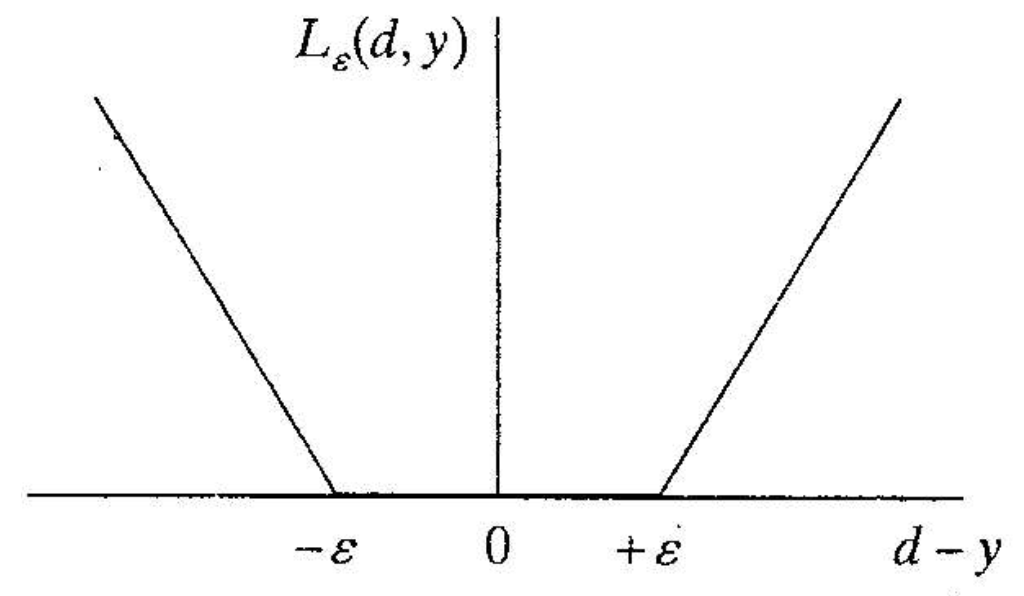
\includegraphics[width=0.5\linewidth]{img/epsiloninsensitive.png}
\end{figure}
By plotting the function and the resulting margin, the $\epsilon$-tube is constructed. (?)

To formulate the optimization problem for regression, we must first introduce two sets of slack variables, $\xi_i'$ and $\xi_i$, such that:
\begin{equation*}
    -\xi_i' - \epsilon \leq d_i - w^T\phi(x_i) \leq \epsilon + \xi_i \,, \forall i = 1, \dots , N
\end{equation*}
We can now formulate the primal and dual problems for regression.

\BoxDef{Quadratic optimization problem for regression (primal form)}{
Given the training set TR = $<x_i, d_i>$, find the optimal values of $w$ which minimize
\begin{equation*}
    \Psi (w,\xi,\xi') = \dfrac{1}{2}w^T w + C \sum_{i=1}^N (\xi_i + \xi_i')
\end{equation*}
satisfying the following constraints
\begin{gather*}
    -\epsilon - \xi_i' \leq d_i - w^T\phi(x_i)  \leq \epsilon + \xi_i \\
    \xi_i \geq 0 \\
    \xi_i' \leq 0
\end{gather*}
}

\BoxDef{Quadratic optimization problem fr regression (dual form)}{
Given the training set TR = $<x_i,d_i>$, find the optimal values of $\alpha_i$ and $\alpha'$ which maximize
\begin{equation*}
    Q(\alpha, \alpha') = \sum_{i=1}^N d_i(\alpha_i - \alpha_i') - \epsilon \sum_{i=1}^N \alpha_i + \alpha_i' - \dfrac{1}{2}\sum_{i,j=1}^N (\alpha_i - \alpha_i')(\alpha_j - \alpha_j')k(x, x_i)
\end{equation*}
satisfying the following constraints
\begin{gather*}
    \sum_{i=1}^N \alpha_i - \alpha_i' = 0 \\
    0 \leq \alpha_i \leq C \\
    0 \leq \alpha_i' \leq C
\end{gather*}
}
Again, solving the dual problem gives us the best values of $\alpha_i$ and $\alpha_i'$, and then we compute the weight vector:
\begin{equation*}
    w = \sum_{i=1}^N (\alpha_i - \alpha_i')\phi(x_i) \iff w = \sum_{i=1}^N \gamma_i \phi(x_i)
\end{equation*}
In this case, the support vectors correspond to non-zero values of $\gamma_i$.

So, the estimate function can be expanded accordingly:
\begin{align*}
    h(x) = y = w^T \phi(x) = \\
    = \sum_{i=1}^N \gamma_i \phi(x_i) \phi(x) = \\
    = \sum_{i=1}^N \gamma_i k(x_i,x) \,.
\end{align*}

\section{Pros and Cons of SVM}

\textbf{Pros:}
\begin{itemize}
    \item The regularization is embedded within the optimization problem, so it does not need any external hyperparameter for it;
    \item It automatically approximates SRM by finding the hypothesis with the best possible VC-dim;
    \item It's a convex problem, so the global minimum can always be found;
    \item Features are implicitly transformed through kernels;
    \item Linear model with bound of the  complexity that depends on the margin (which is optimized);
    \item Rich set of non-linear decision functions in the input space via kernels.
\end{itemize}

\textbf{Cons:}
\begin{itemize}
    \item Kernel and kernel parameters must be chosen explicitly;
    \item It uses a batch algorithm to update the weights, so no chance to parallelize;
    \item Very large problems were computationally intractable (although nowadays many efficient solutions have been proposed, including gradient descent ones);
    \item For soft margin SVM, since we have to select the $C$ parameter and the kernel function, we have no guarantee that the final model will have high accuracy.
\end{itemize}

Note that for the last point about soft margin, the VC-dim of the model is controlled by the width of the margin. If we choose the smallest possible margin (with just one support vector), we can classify an arbitrarily large number of training points correctly, thus the VC-dim will be infinite. If instead we have a very large width, we end up in a situation where all points in the TR set are used as support vectors, therefore leading to a low VC-dim. This is analogous to using a k-NN classifier with $k=1$ and $k=l$, respectively. Also, the hyperparameter $C$ used for regularization must be chosen appropriately for the kernel hyperparameters, so cross-validation is needed.

\section{Kernel Methods}

In general, \textbf{kernelization} of an approach is done by substituting a dot product or similarity measure in a model with a kernel function that maps to an high-dimensional space.

$K(s,t)$ can be related to a similarity measure, comparing $s$ and $t$; e.g.:
\begin{equation*}
    d_k(s,t) = \sqrt{k(s,s) - 2k(s,t) + k(t,t)}
\end{equation*}
If the objects are similar (so the distance is small) the kernel will have high value. The focus is on the idea that in some situations, it's easier to focus on simplifying pairwise comparison by doing it in a different space rather than the representation of the single object.

The best choice of kernel for a given problem is still a research issue.
\chapter{Bias, Variance, and Ensembling}

A model is trained on the basis of a specific training dataset containing a finite number of instances. Each training set is only one of the possible realizations of the universe of data obtained through empirical measurements, so different training sets can provide different estimates. When determining the error of a model, noise should be taken into consideration. This chapter will focus on the different aspects that influence the quality of the final model.

\section{Bias, Variance, Noise}

The expected error of the model at a point $x$ can be decomposed as:
\begin{itemize}
    \item \textbf{Bias}: it quantifies the inability of the model to accurately approximate the target function. It can be seen as an approximation error.

    \item \textbf{Variance}: it quantifies the variability of the response of the model for different realizations of the training data. It can be seen as an estimation error.

    \item \textbf{Noise}: it's a random error included in a label in the training set, caused by imperfect measurements. It's irreducible, since it does not depend on the model.
\end{itemize}

Assume we have a regression task, where the target variable is $y$ and we use the squared error loss $L_2$. Our training set is TR = $< x, y >$, where $y = f(x) + \epsilon$, and $\epsilon$ is Gaussian noise with 0 mean and standard deviation $\sigma$. We fit a linear hypothesis $h(x) = w_1x + w_0$ to minimize the SSE over the training data. We will have a systematic prediction error, since the model is not flexible enough to approximate certain target functions (e.g. second degree functions). Also, depending on the dataset, the $w$ parameters will be calculated differently.

So, given a new data point $x$, what is the expected prediction error? Assume that all the data points are drawn from a set of independent and identically distributed variables with the same probability distribution $P$. The goal is to compute, for any new $x$:
\begin{equation*}
    E_p [(y-h(x))^2] \,,
\end{equation*}
where $y$ is the value of $x$ that can be found in a dataset, and the expectation is over all training sets drawn according to $P$.

Let $Z$ be a random variable with possible values $z_i, \, i = 1 \dots l$ and probability distribution $P(Z)$. Its \textbf{expected value (mean)} is:
\begin{equation*}
    \Bar{Z} = E_p[Z] = \sum_{i=1}^l z_iP(z_i)
\end{equation*}
If $Z$ is continuous, the sum is replaced with an integral, and the distribution function by a density one. The \textbf{variance} of $Z$ is:
\begin{equation*}
    Var[Z] = E[(Z - \Bar{Z})^2] = E[Z^2] - \Bar{Z}^2 \,.
\end{equation*}
The proof of this last equality is the following:
\begin{gather*}
    Var[Z] = E[(Z - \Bar{Z})^2] = \sum_{i=1}^l (z_i - \Bar{Z})^2 P(z_i) = \\
    = \sum_{i=1}^l (z_i^2 - 2 z_i \Bar{Z} + \Bar{Z}^2) P(z_i) = \sum_{i=1}^l z_i^2 P(z_i) - \sum_{i=1}^l 2 z_i \Bar{Z} P(z_i) + \sum_{i=1}^l \Bar{Z}^2 P(z_i) = \\
     = E[Z^2] - 2\Bar{Z} \sum_{i=1}^l z_i P(z_i) + \Bar{Z}^2 \sum_{i=1}^l P(z_i) = E[Z^2] - 2 \Bar{Z} \Bar{Z} + \Bar{Z}^2 \cdot 1 = \\
     = E[Z^2] - 2 \Bar{Z}^2 + \Bar{Z}^2 = E[Z^2] - \Bar{Z}^2 = Var[Z]
\end{gather*}
We will use the form $E[Z^2] = \Bar{Z}^2 + Var[Z]$ (variance lemma).

The error can be rewritten as:
\begin{equation*}
    E_p[(y - h(x))^2] = E_p[h(x)^2 - 2yh(x) + y^2] = E_p[h(x)^2] + E_p[y^2] - 2E_p[y]E_p[h(x)]
\end{equation*}
Let $\Bar{h}(x) = E_p[h(x)]$ be the mean prediction of the hypothesis at $x$ when $h$ is trained on data drawn from $P$. Using the variance lemma defined above, we can rewrite the squared error as:
\begin{gather*}
    E_p[(y - h(x))^2] = \Bar{h}(x)^2 + E_p[(h(x) - \Bar{h}(x))^2] + f(x)^2 + E_p[(y - f(x))^2] - 2f(x)\Bar{h(x)} = \\
    = E_p[(h(x) - \Bar{h}(x))^2] + \Bar{h}(x)^2 - 2f(x)E_p[h(x)] + f(x)^2 + E_p[(y - f(x))^2] = \\
    = E_p[(h(x) - \Bar{h}(x))^2] + \textbf{(variance)}\\
    + (\Bar{h(x)} - f(x))^2 + \textbf{(bias$^2$)} \\
    + E_p[(y - f(x))^2] = \textbf{(noise$^2$)} \\
    = Var[h(x)] + Bias[h(x)]^2 + E_p[\epsilon^2]
\end{gather*}
(the mean of $y$ is $f(x)$).

\subsection{Regularization}

Recall how we implemented regularization to calculate the loss function:
\begin{equation*}
    Loss(w) = \sum_p (d_p - o(x_p))^2 + \lambda \|w\|^2
\end{equation*}
By varying the value of the regularization hyperparameter $\lambda$, we ca obtain more or less complex solutions. Consider the following graphical examples to understand how it affects bias and variance of the model; the training sets here are taken from a sinusoidal distribution.

\begin{figure}[H]
    \centering
    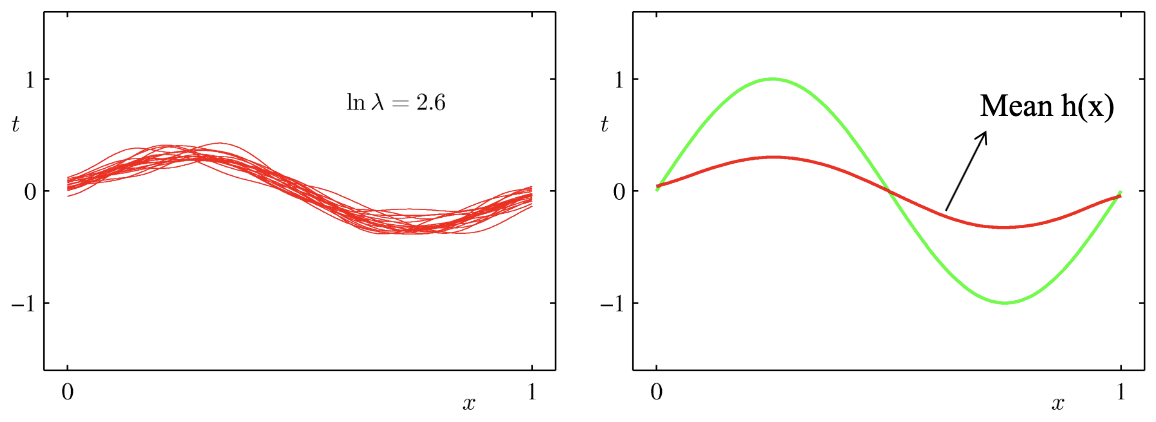
\includegraphics[width=0.9\textwidth]{img/BiasVar1.png}
    \caption{High lambda, high bias, low variance. Not too dependent on data, but the model is too rigid. The model underfits the data.}
\end{figure}
\begin{figure}[H]
    \centering
    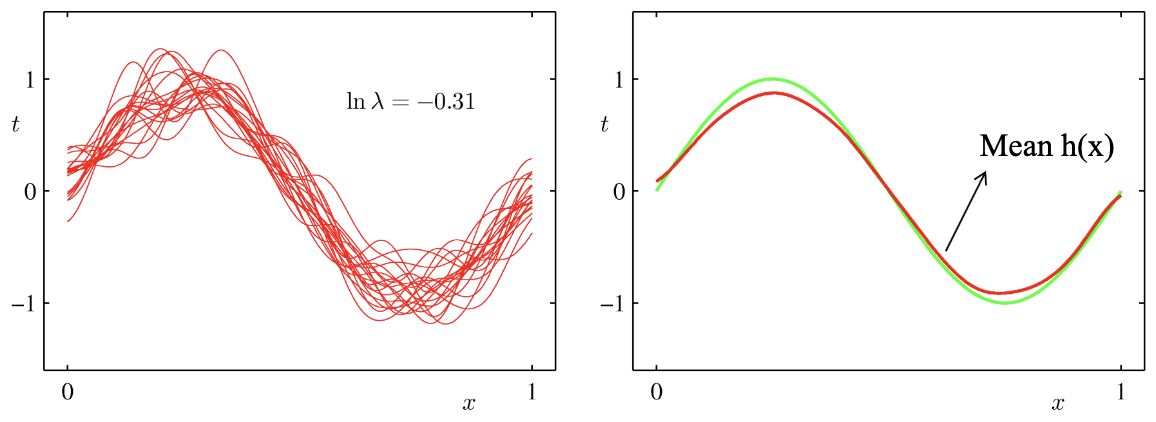
\includegraphics[width=0.9\textwidth]{img/BiasVar2.png}
    \caption{Low lambda, low bias, high variance. The model is more dependent on training data, but approximates better.}
\end{figure}
\begin{figure}[H]
    \centering
    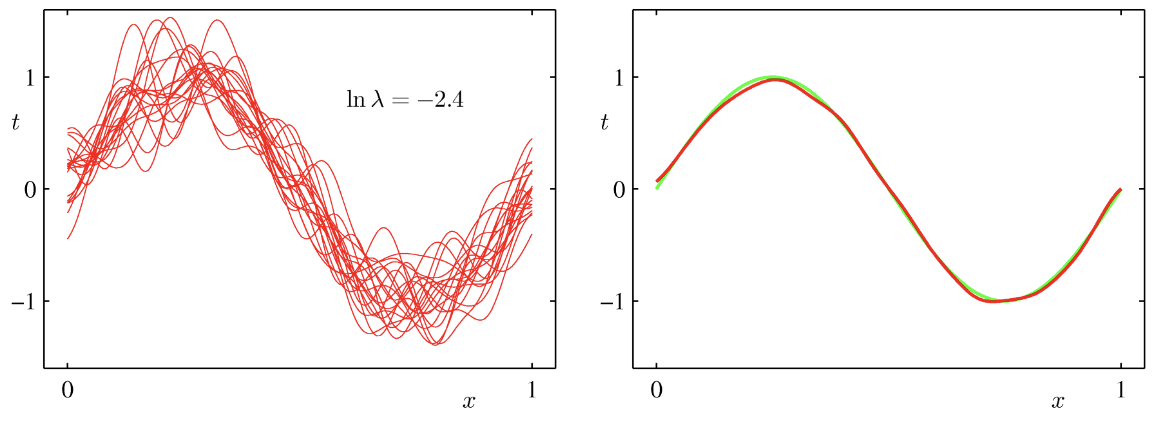
\includegraphics[width=0.9\textwidth]{img/BiasVar3.png}
    \caption{Very low lambda, very low bias, very high variance. Final hypothesis may produce an high test error. The model overfits the data.}
\end{figure}
This highlights once again how the goal of model selection is to find the best trade-off between model complexity (bias) and training error (variance).

\section{Ensemble learning}

Ensemble learning estimates the output of an instance by considering the prediction of multiple models trained differently instead of just one.

The simplest case is \textbf{voting}. All models are trained on the same training set. For regression, the simple average committee of the models is calculated:
\begin{equation*}
    o(x) = \dfrac{1}{K} \sum_{k=1}^K h_k(x)
\end{equation*}
The square error of a committee is less or equal than the mean of the square errors. For classification, we use different classifiers and take the majority vote (or the instance is classified after calculating the mean of the continuous outputs).

Another scheme is \textbf{bagging} (also called \textbf{bootstrap aggregating}). $K$ models are trained on different subsets of the training set, and each training is differentiating using bootstrap (so resampling with replacement). For regression, the final prediction will be the mean, while for classification we consider the majority vote.

If models have the same errors, however, we will not have any advantage in using ensembling. A solution is \textbf{boosting}: we first differentiate each training in order concentrating on errors, so we give more weight to ``difficult'' instances, such as ones that get misclassified by the previous classifier. The results are then combined in the output weights. If not stopped, boosting will learn to classify correctly all training instances, even when given a set of weak learners that are barely better than a random guesser. Even if bias is reduced, variance does not increase, so it resists well to overfitting (although it's not immune). However, it's sensitive to noisy data, since it will be deemed ``difficult'' and therefore receive an heavier weight.


\chapter{Deep Learning}

\section{Convolutional Neural Networks}

Convolutional Neural Networks are a specialized kind of neural network for processing data with a known, grid-like topology, such as 2D images. The name ``convolutional'' refers to the usage of the mathematical operation called \textbf{convolution}, indicated by an asterisk ($*$). This is an operation of two functions of a real valued argument, defined as follows:
\begin{equation*}
    s(t) = (f * g)(t) \stackrel{def}{=} \int_{-\infty}^{\infty} f(\tau)g(t - \tau) d \tau = \int_{-\infty}^{\infty} f(t - \tau)g(\tau) d\tau \,,
\end{equation*}
The idea behind this operator is that we want to calculate the average of $f$ weighted by another function $g$ moved over time (``sliding''), calculated for a certain $t$. In convolutional network terminology, the first argument (here, $f$) is referred to as the \textbf{input}, and the second argument ($g$) as the \textbf{kernel}. The output is called \textbf{feature map}.

This operator can be applied to neural networks as well. Consider a simple network with one hidden layer:
\begin{figure}[ht]
    \centering
    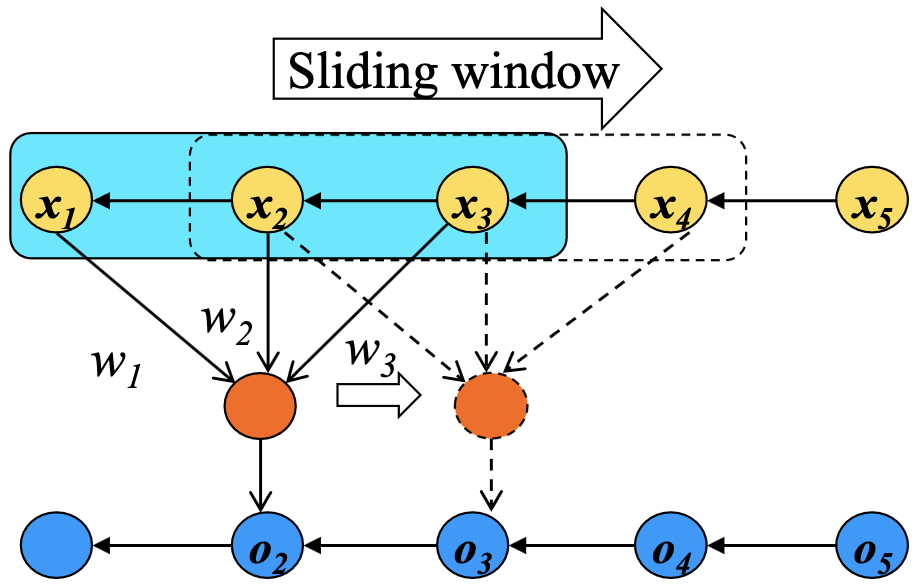
\includegraphics[width=0.45\linewidth]{img/CNN_simple.png}
\end{figure}

Here, the output of each node in the hidden layer is calculated as $out_t = \sum_{i=1}^3 w_i x_{t+i-2}$. In other words, the weights assigned to the inputs ``slide'' across the hidden layer. Weights are tuned as usual by learning.

\subsection{2D Convolution}

Discrete convolution can be seen as a multiplication by a matrix, with several entries constrained to be equal to other entries. The convolution over a 2D image $I$ with a kernel $K$ can be expressed as:
\begin{equation*}
    S(i,j) = (I*K)(i,j) = \sum_m \sum_n I(m,n)K(i-m, j-n) \,,
\end{equation*}
or, as expressed by many libraries, as the \textbf{cross-correlation function}:
\begin{equation*}
    S(i,j) = (I*K)(i,j) = \sum_m \sum_n I(i+m,j+n)K(m, n) \,.
\end{equation*}

The example below shows a 2D image with 25 pixels, and a 3x3 kernel (unit local receptive field) with a stride equal to 1 (i.e., the kernel moves across the image 1 pixel at a time; by choosing the stride we choose the size of the feature map). The image also has padding added to its edge.
\begin{figure}[ht]
    \centering
    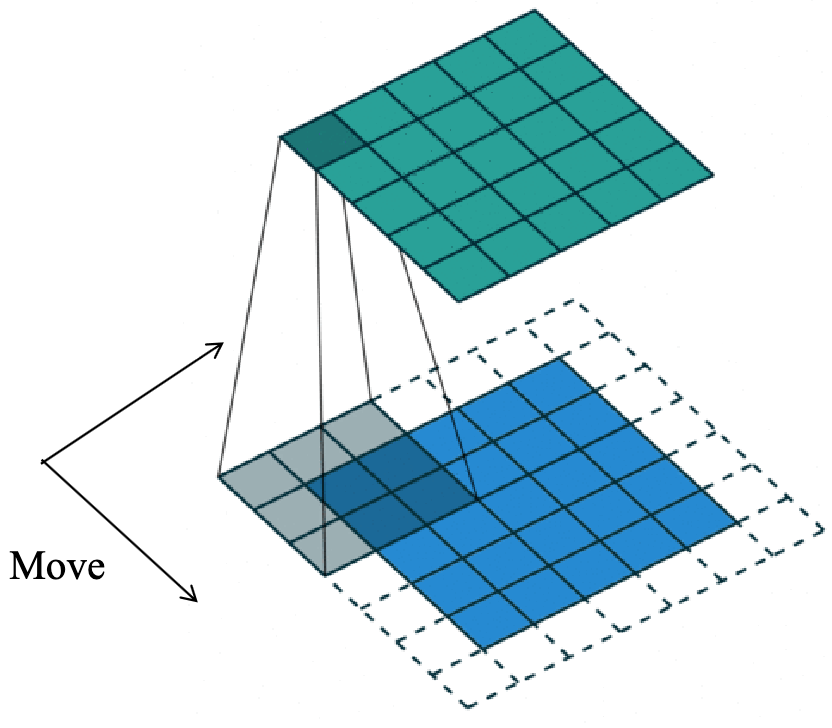
\includegraphics[width=0.6\linewidth]{img/CNN_2D.png} 
\end{figure}

Once the kernel reaches the end of the first ``row'' of pixels, it restarts from the position it started from shifted one pixel below. The full movement of the kernel over the image produces the feature map.

The image below better shows the matrix multiplication interpretation of convolution; the image is 4x3 and the kernel is 2x2. The stride is again equal to 1.

\begin{figure}[ht]
    \centering
    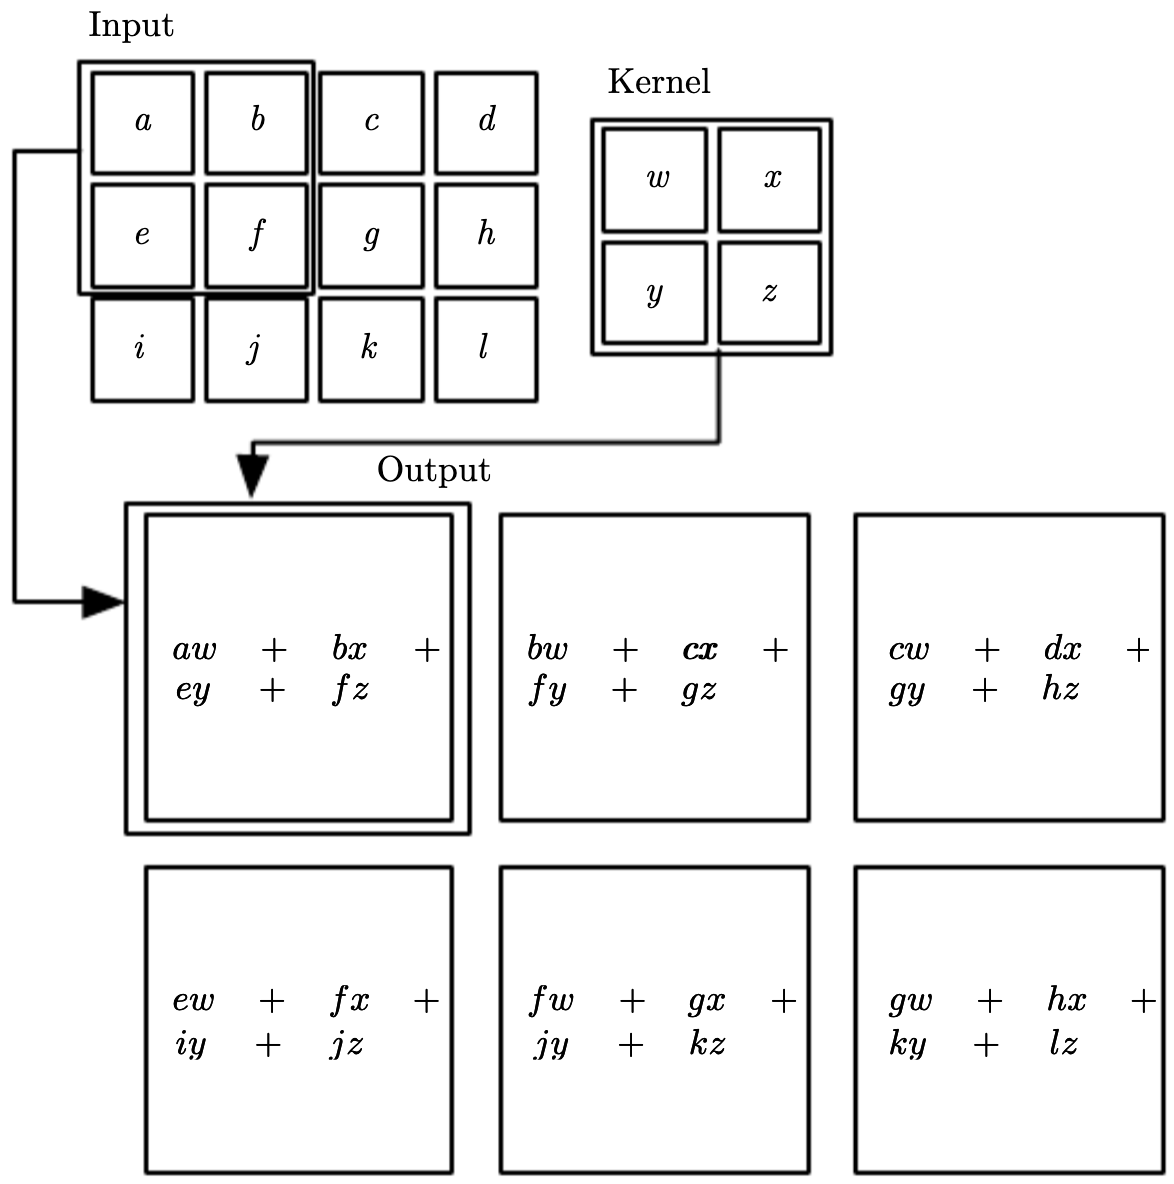
\includegraphics[width=0.5\linewidth]{img/CNN_matrix.png}
\end{figure}
Each unit's weights are a \textbf{filter} trained to detect some specific feature or pattern in the image. Each filter produces the strongest response to a spatially local input pattern, and then the filters obtained by training are applied to the whole (global) image, so that features and patterns can be identified regardless of where they are positioned on the image.

The size of the feature map can be reduced via pooling. Some examples of pooling are:
\begin{itemize}
    \item Subsampling, using a stride greater than 1;
    \item Calculating a mean (average or weighted average);
    \item Using the max pool operation (most common option).
\end{itemize}
This way, instead of producing a value for every single pixel of the original image, we get a smaller set of pixels where each value is obtained by considering the values of neighboring ones (calculating the mean or max value). Pooling also helps to make the representation approximately invariant to small translations of the input, since the mean or max value of a neighborhood of points is unlikely to be affected by a small translation of the pixels in the image.

CNN exploits \textbf{weight sharing}, where the number of connections in the network is kept the same while reducing the number of actual free parameters. The produced sliding window of units is applied over a segment of the input, and reapplied multiple times to produce various layers of feature maps. Training of the weights is usually done via backpropagation. Since these networks tend to be big and deal with large amount of data, many hyperparameters are fixed by experience or by suggestions of experts, since it would be too expensive to run cross-validation.

\section{Deep Learning}

The Deep Learning framework includes many different models, such as:
\begin{itemize}
    \item Deep Neural Networks;
    \item Convolutional Neural Networks;
    \item Deep belief Networks;
    \item Recurrent and Recursive Neural Networks.
\end{itemize}
They differ from ``shallow'' models in that they have a big amount of layers.

There's many different approaches to build a deep learning model. All these approaches have some aspects in common:
\begin{itemize}
    \item Multiple layers of nonlinear processing units;
    \item Supervised or unsupervised learning of feature representation in each layer, with the layers forming some hierarchy from low to high level features;
    \item Hierarchical sparse/distributed representation of the input data.
\end{itemize}

The core concept at the base of deep learning is increasing the level of abstraction of the data through the use of several layers; for example, an image can be gradually abstracted on each layer, first as a vector of intensity values per pixel, then a set of edges, then regions of a particular shape, and so on. We've already mentioned this idea with CNNs: the original complicated mapping is broken down into its simple elements, by gradually calculating simpler mapping at each layer. A series of hidden layers extracts increasingly abstract features from a set of example images. Additionally, these abstract features, once learned by the units, can also be combined together to generalize on examples that were never seen during training.

In general, deeper networks are often able to use less units per layer, thus less free parameters as well and less training data required to achieve a good generalization. Still, many layers may be harder to be trained, so there's a need to improve the techniques we know regarding gradient descent, regularization, and data exploitation.

\subsection{Insights}

\subsubsection{Why So Many Layers?}

Imagine a two-layer circuit of logic gates, which can represent any Boolean function. Any Boolean function can indeed be written as a sum of products (i.e., in disjunctive normal form). With logical circuits of depth two, the number of logic gates required to represent most Boolean functions is exponential w.r.t. input size.

An example of such function is the parity function: it returns 1 if there is an odd number of 1s over $N$ binary inputs (i.e., $N$ bits), 0 otherwise. If we were to implement this function with logic gates, assuming $N$ inputs, we would need:
\begin{equation*}
    \dfrac{2^N}{2} + 1 = 2^{N-1} + 1
\end{equation*}
gates, since we have to perform 1 OR and exactly $2^{N-1}$ ANDs.

We can propose an alternative solution with a polynomial number of gates, by increasing the number of layers to $log(N)$. The solution for $N=8$ is shown below (in a simplified view where each XOR corresponds to 2 AND gates and 1 OR gate). In this solution, the number of gates is greatly reduced from $2^7 + 1 = 129$ to only $7 * 3 = 21$.
\begin{figure}[ht]
    \centering
    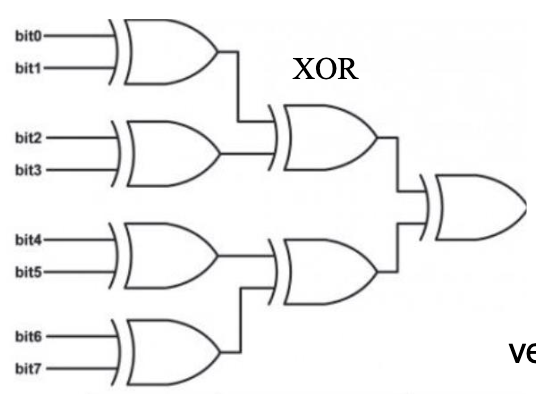
\includegraphics[width=0.5\linewidth]{img/Circuit_deep.png}
\end{figure}

The universal approximation theorem states that even with 1 hidden layer, a NN can approximate any possible function, however it does not specify the number of units needed. For some families of functions a boundary on this number can be found, but as seen in the example above, the bound may be exponential w.r.t. the dimension of the input. Also, there exist families of functions which can be approximated efficiently by a NN with depth greater than some value $d$, but which require a much larger model if depth is restricted to be less or equal than $d$.

This theorem also implies that regardless of what function we are trying to learn, a large MLP is able to represent the function, but there's no guarantee that that the training algorithm will be able to learn that function, either because it can't find the value of the parameters that correspond to the desired function, or because it might choose the wrong function due to overfitting. So another advantage to using multiple layers is ensuring that the learning algorithm can actually properly learn.

The inductive bias is: choosing a deep model encodes the (very general) belief that the function we want to learn should involve composition of several simple functions. If our task actually matches our bias, then the deep shape of the learner is suitable, and those deeper models also perform better than shallow ones. Typically, these tasks are the ones that involve images or language, but for other tasks that deal with different data this deep structure may not be appropriate.

Other challenges that motivate the usage of deep neural networks are related to the curse of dimensionality and manifold learning.

Recall that the curse of dimensionality is the phenomenon in which as the number of dimensions in the data increases, the less dense it is, thus becoming a problem for distance based machine learning algorithms. One challenge posed by this phenomenon is a statistical one: this challenge arises when the number of possible configurations of an input $x$ is much larger than the number of actual training examples. Let's say we want to estimate the probability density for some point $x$ by returning the number of training examples in the same unit volume cell as $x$ divided by the size of the training set. But if we want to estimate this density for a point that has no close neighbors within the unit volume cell (as is often the case when the dimensionality of data is high), there's no immediate way to calculate it. Additionally, even if present, neighbors are likely going to be very few. But deep learning is the solution: it can learn the single features it identifies in the training data, and those features can then be combined to produce an output even for instances that were never seen before.

A manifold is a connected region. Mathematically, it's a set of points associated with a neighborhood around each point. From any given point, the manifold locally appears to be a Euclidean space. As an example, in the real world, we experience the surface of the Earth as 2D, but in reality it's a sphere in 3D space. In the case of Machine Learning, ``manifold'' is a term used to broadly refer to a connected set of points that can be approximated well by considering only a small number of dimensions. Different points can also have a different number of dimensions, typically when the manifold intersects itself. \textbf{Manifold learning} assumes that the only interesting inputs occur only along a collection of manifolds containing a small subset of points, with interesting variations in the output occurring only across directions that lie on the manifold, or only when moving from one manifold to the other. This assumption is often used for data types such as images, text, or audio that occur in real life, since uniform, artificial noise never resembles the inputs from those domains, so the probability distribution of the only valid data is highly concentrated. *?

\subsubsection{Representation Learning}

With Deep Learning, other concepts are emerging, such as representation learning, which is the set of methods that automatically discover the best representation of raw data for some other task. It's especially useful for more complex data types like images, text, or audio data. Deep Learning methods are also representation learning methods with multiple levels of representation.

The reason behind representation learning is that many information processing tasks can have varying difficulty based on the way the information is represented. In Machine Learning, a good representation is one that makes a subsequent learning task easier. Supervised learning in MLPs is an example that leads to an automatic representation at every hidden layer taking on properties that make the output layer task easier (think of the XOR example). Another example is CNNs, since they take as input a raw image and automatically learn to identify the main features of the image, decomposing it into its parts.

The hidden representation of data can be obtained via \textbf{pretraining approaches}, semi-supervised learning, which means we can learn a representation for the unlabeled data and use it to solve supervised tasks. The representation can be then exploited with \textbf{transfer learning} approaches.

\paragraph{Pretraining}

\textbf{Greedy Layer-Wise Unsupervised Pretraining} was the first approach to make it possible to train a deep supervised network. It makes the training of the whole network much easier, since there's no need for an end-to-end training from the output layer to the previous hidden layers with a gradient descent, which used to be difficult for deep models. The adjective ``greedy'' refers to the fact that each layer is optimized independently in an unsupervised way. This methods works not only as a good initialization strategy, but also as regularization regarding the complexity of the original data, since it extracts the features that simplify the unsupervised process. It also reduces the variance of the estimation training process, since pretrained models tend to gather in a smaller region after training).

\paragraph{Autoencoders}

An autoencoder is a neural network that is trained to attempt to copy its input to its output. It has a hidden layer $h$ that describes a \textbf{code} used to represent the input. The network can be seen as two components: the encoder function $h = f(x)$, and the decoder $r = g(h)$ that produces a reconstruction. Autoencoders are specifically trained so that they are unable to copy the input perfectly, but instead only copy parts of the data or copy it only approximately. Since the model is forced to prioritize only some aspects of the input, it often learns useful properties of the data.

Autoencoders can be:
\begin{itemize}
    \item \textbf{Undercomplete}, if the code dimension is less than the input dimension. This autoencoder is forced to learn the salient features of the training data by the constraints in the architecture itself.

    \item \textbf{Overcomplete}, if the code dimension is greater than the input dimension. By itself the autoencoder would learn to copy the input as is, so some form of regularization is needed to introduce constraints in the sparsity of the representation, robustness in the noise, and other properties of interest.
\end{itemize}

A commonly used type of autoencoders are denoising autoencoders. They are trained on a set of images, finding the best representation of them (the one they can obtain even from corrupted/noisy data). Once they are presented with an image with added noise, they are capable of reconstructing the original.

Stacked autoencoders are multiple autoencoders stacked on top of each other. The algorithm used to train a stacked autoencoder is the following:
\begin{enumerate}
    \item Train the first layer as an autoassociator (i.e., an autoecoder whose input and output are the same), in order to minimize the reconstruction error of the raw input;

    \item The hidden units' outputs in the autoassociator are now used as input for another layer, also trained to be an autoassociator. Repeat this step until the desired number of layers is reached.

    \item Take the last hidden layer output as input to a supervised layer, and initialize only its parameters (randomly or by supervised learning).

    \item Fine-tune all the parameters of the architecture with respect to the supervised criterion.
\end{enumerate}

The idea is that the unsupervised greedy layer-wise initialization put all the parameters of all the layers in a region of parameter space from which a local optimum can be reached via local descent.

In the past, pretraining acted as the start of Deep Learning. It can yield improvements for some tasks, especially NLP, but not in others. The general role of pretraining is nowadays under critical revision by researchers.

\paragraph{Transfer Learning}

\textbf{Transfer learning} refer to the situation where what has been learned in one setting is used to improve generalization in another setting. In this case, we use the best representation of the data found by pretraining to improve the generalization capabilities of some model. In \textbf{domain adaptation}, the task remains the same between each setting, but the input distribution is different. With \textbf{multi-task learning}, a trained model can be used for a task that's different from the one it was trained for (it will receive the same inputs, but the target variable(s) change).

\subsubsection{Distributed Representation}

As opposed to \textbf{symbolic representation}, in which each input corresponds to an unique symbol, in \textbf{distributed representation} each input is represented by a set of elements that can be set separately from each other. As an example, consider a vector of $n$ binary features, which can take $2^n$ possible configurations, each corresponding to a different region in input space. This is a type of distributed representation. The same data can be represented via one-hot encoding: $n$ feature detectors, each corresponding to the detection of a certain input. Only $n$ configurations of the input space are possible. This is a type of symbolic representation. The two representations are visualized below.

\begin{table}[ht]
    \centering
    \begin{tabular}{|c|cccc|}
        \hline
        \rowcolor{gray}
        Input & barks & hasFur & hasLegs & isFruit \\
        Dog & 1 & 1 & 1 & 0 \\
        Cat & 0 & 1 & 1 & 0\\
        Apple & 0 & 0 & 0 & 1\\
        Kiwi & 0 & 1 & 0 & 1\\
        \hline
    \end{tabular} 
\quad
    \begin{tabular}{|c|cccc|}
        \hline
        \rowcolor{gray}
        Input & isDog & isCat & isApple & isKiwi \\
        Dog & 1 & 0 & 0 & 0 \\
        Cat & 0 & 1 & 0 & 0 \\
        Apple & 0 & 0 & 1 & 0 \\
        Kiwi & 0 & 0 & 0 & 1 \\
        \hline
    \end{tabular}
    \caption{Distributed representation on the top, symbolic representation on the bottom.}
\end{table}

In distributed representation, values assigned to attributes can also be real-valued. By using this representation, we can calculate similarity between two different concepts (inputs); in symbolic representation, the distance between two inputs is always $\sqrt{2}$.

In general, distributed representation is used in input only if we have background knowledge (one-hot encoding is used instead), while it is commonly used automatically during learning. A big advantage is that there's no need to characterize all the possible configurations of the input, but only the distinction across specific concepts (e.g., in the example above, we learn the characteristics ``barks'', ``hasFur'', ``isFruit'' instead of learning exactly what a dog or an apple are).

Sharing attributes among inputs allows the model to both treat them similarly, and automatically learn such similarity. As per the example above, ``dog'' and ``cat'' share some features. If we are presented with textual data containing several different words, and by learning the model knows the similarity between ``cat'' and ``dog'', a sentence that contains the word ``cat'' can inform the predictions made for a sentence containing the word ``dog'', and vice-versa. Since they're represented in a distributed way, the distance between the two is actually measurable and comparable with respect to other inputs (e.g., ``dog'' is closer to ``cat'' but both are further away from ``apple'', while with one-hot-encoding their distance is $\sqrt{2}$ regardless of how similar the concepts represented by those words are).

One drawback of distributed representation is that it's more difficult to interpret.

\subsection{Techniques}

When implementing a deep neural network, there's many technical aspects to consider. As already stated before, the deeper the network, the less units are needed for each layer, and therefore there will be less parameters to train, but some layers may be difficult to train. This section will focus on the methods that need improvement and their issued when used with deep NNs.

The first issue is related to the gradient. With deep NNs, there's now a lot of layers to backpropagate the gradient through. If the weights are too small, they will shrink exponentially (gradient vanish), while if they are too big, they will grow exponentially. This happens because the repetition of multiplication through many layers can introduce cliffs in the cost functions, that when traversed will drastically increase or decrease the weights. One solution is using \textbf{gradient clipping}: if the norm of the gradient $\|g\|$ is greater than some threshold $v$, then $g = v*\frac{g}{\|g\|}$, so the movement towards the gradient direction still happens, but the weight updates are bounded.

For gradient vanish, traditional activation functions have gradients in the range $[-1,1]$, and backpropagation computes gradients via chain rule repeated through layers. This means that for each layer, the gradient of the layer in the front will be multiplied by a value $d,\,|d| \geq 1$, so the layers closer to the input will be trained much more slowly. There are many approaches to deal with it, one of which is using the \textbf{ReLU (Rectified Linear Unit)} activation function:
\begin{equation*}
    f(x) = \max(0,x)
\end{equation*}
This function makes it so that the derivative of a unit remains large as long as the unit is active. *?

\textbf{Batch normalization} is a method that normalizes each batch by calculating each individual batch statistics such as mean and variance for each layer. Each matrix (batch x activation of units) is normalized with mean and variance, shifting the values to zero-mean and unit variance. This technique helps to keep the normalization of the input across all layers of the network. It also achieves a faster learning and higher accuracy for Deep Learning.

\textbf{Dropout} is a method that makes bagging more practical for large neural networks. Bagging involves training multiple models on different subsets of the data, and then evaluating multiple models on the same test example. Dropout trains the ensemble consisting of all sub-networks that can be formed by removing non-output units from an underlying base network. In most modern neural networks, we can effectively remove a unit from a network by multiplying its output value by 0. Then, a minibatch-based learning algorithm is used to train one working sub-network at a time. The sub-network is selected at random, with each binary mask to apply to the original network having a different probability set as an hyperparameter (e.g., 0.8 for input units and 0.5 for hidden units). The sub-networks inevitably share weights, since they're obtained from the same base network; this causes the training of the sub-networks to find good settings for the parameters.

Dropout has a regularization effect as well: it avoids to train all units on all training data and reduces unit interactions. It also reduces variance without affecting bias just like bagging does. It even regularizes singular hidden units to be not just good features, but features that can be good in different contexts (different sub-networks). It can be used for any model that uses distributed representation and SGD training.
\chapter{Randomized Machine Learning}

Randomness can be seen as an effective part of Machine Learning approaches. It can enhance different aspects, such as data processing, learning, hyper-parameter selection, and so on. It can both enhance predictive performance and alleviate difficulties of classical ML methodologies.

Randomness can also be exploited to reduce the training needed for a MLP/RNN, by implementing \textbf{randomized neural networks} (or \textbf{random weights neural network}). The network is constructed with randomly connected hidden layers with fixed weights. The training involves only the output weights, overcoming the problems associated with the typical training algorithms used for neural networks. The general architecture of a randomized NN is defined by two components:

\begin{itemize}
    \item The hidden layer (untrained, randomly initialized). It linearly embeds the input into a high-dimensional feature space where the problem is more likely to be solved linearly.

    \item The readout layer (trained). It combines the features in the hidden space for output computation.
\end{itemize}

\textbf{Cover's theorem} states: ``a complex pattern-classification problem, cast in a high-dimensional space nonlinearly, is more likely to be linearly separable than in a low dimensional space, provided that the space is not densely populated''.

\section{Pros and Cons}

A large set of hidden units can provide a sufficient ``basis expansion'' to project the non-linearly separable data into an higher dimension, and is also extremely efficient at doing so.

On the other hand, focused models with a smaller number of adaptive units trained on the specific task at hand wiill appear more ``elegant''.

\nocite{*}
\bibliographystyle{plain}
\clearpage\bibliography{bibliography}

\end{document}
